\documentclass[drones,article,submit,moreauthors]{Definitions/mdpi}

\usepackage{amsmath}
\usepackage{amssymb}
\usepackage{algorithm}
\usepackage{algpseudocode}
\usepackage{booktabs}
\usepackage{graphicx}
\usepackage{subcaption}

\firstpage{1}
\makeatletter
\setcounter{page}{\@firstpage}
\makeatother
\pubvolume{1}
\issuenum{1}
\articlenumber{0}
\pubyear{2026}
\copyrightyear{2026}
\datereceived{ }
\daterevised{ }
\dateaccepted{ }
\datepublished{ }

\Title{AeroMesh, a Self-Healing Aerial Edge Mesh for Post-Disaster Connectivity and On-Board Damage Assessment in Southeast Asia}

\Author{Anonymous Author(s)}

\AuthorNames{Anonymous}

\address{%
Anonymized for review}

\corres{Correspondence: anonymized for review}

\abstract{Terrestrial networks in Southeast Asia repeatedly fail during the typhoons, earthquakes, and monsoon floods that make connectivity most valuable, cutting off responders and the imagery decision makers need. We propose AeroMesh, a self-organizing aerial mesh of unmanned aerial vehicles providing priority-differentiated connectivity alongside on-board edge inference for building-damage assessment from degraded imagery. Our central claim is that connectivity restoration and damage assessment should be co-designed rather than stacked as independent layers, since the choice of which vehicle relays and which senses must be re-solved as batteries drain and imagery quality fluctuates. We formalize this as a stochastic online optimization solved by three decentralized control loops for mesh formation, role auctioning, and uncertainty-aware early-exit inference with cross-mesh deferral. A completed packet-level ns-3 campaign across 52 of 54 scenario cells spanning named Philippine, Indonesian, and Vietnamese disaster corridors shows AeroMesh matching or exceeding two routing baselines on responder-class delivery in two of three scenarios, with one civilian-class weakness reported alongside the favorable results rather than omitted. A trained early-exit damage classifier evaluated under a corruption pipeline and bidirectional cross-dataset transfer shows substantial accuracy drops under transfer, 70.3 to 42.3 percent and 83.7 to 34.4 percent, while split-conformal coverage degrades only modestly as raw prediction confidence becomes markedly less trustworthy. A reduced-fidelity co-simulator coupling these two layers through the auction does not show AeroMesh dominating a fixed-role ablation on the resulting connectivity-assessment frontier, a finding corroborated by a real joint ns-3 simulation for one of the three scenarios, which we report together with the specific structural reason it should not yet be read as a settled verdict on the paper's central co-design claim.}

\keyword{unmanned aerial vehicles; disaster response; self-healing networks; flying ad hoc networks; edge inference; uncertainty quantification; Southeast Asia; post-disaster communication; damage assessment; connectivity maintenance}

\begin{document}

\section{Introduction}
\label{sec:intro}

Southeast Asia sits on three overlapping hazard corridors at once. The Philippines lies in the Pacific typhoon belt and along the Pacific Ring of Fire, so it experiences both strong tropical cyclones and frequent seismic activity in the same set of provinces. Indonesia straddles three tectonic plates and experienced two near-simultaneous disasters in 2018 when the Lombok earthquake sequence and the Palu earthquake and tsunami struck within weeks of each other \cite{sulawesi2018eq}. Vietnam, Myanmar, and Thailand sit along the Mekong river system, where monsoon flooding regularly isolates whole districts for days at a time. In every one of these events the first resource to fail is the same one that responders most need, which is the communications network that would let them coordinate.

This is not a hypothetical risk. Typhoon Odette, known internationally as Rai, made landfall across twenty-two Philippine provinces in December 2021 and telecommunications operators reported that the outage was caused by multiple fiber cable cuts after utility poles carrying the cables collapsed \cite{odette_telecom_2022}. The national telecommunications department had to form a dedicated task force to restore the downed lines \cite{odette_dict_2021}, and a local official in Mindanao argued publicly that the deeper problem was insufficient resiliency investment by the telecommunications companies themselves \cite{mindanao_resiliency_2021}. A different and larger-scale failure mode struck the whole region in December 2006, when two earthquakes near the Luzon Strait triggered a submarine landslide that severed the majority of the submarine cable systems running through that strait at depths where repair vessels could not operate quickly \cite{luzon_cable_2006,nanog_taiwan_cable}. That single event interrupted the majority of voice, data, and internet traffic across Southeast Asia for days, and analysts attributed part of the damage to the fact that most of the region's cable routes run in the same earthquake-prone direction rather than along diverse paths \cite{sulawesi_cable_risk}. More recently, Typhoon Yagi in 2024 severed seven inter-provincial fiber routes and twelve intra-provincial transmission lines in Vietnam and knocked more than a hundred base stations offline in a single province \cite{yagi_vietnam_2024}. These are not isolated incidents. They are the recurring signature of a region where terrestrial and submarine infrastructure share the same geography as the hazards that threaten it.

Unmanned aerial vehicles carrying communication payloads are an established response to exactly this kind of failure. Early field demonstrations showed that a handful of drones carrying commodity Wi-Fi radios could restore multi-hop connectivity over hundreds of meters per hop \cite{panda2019design}, and unmanned aerial vehicle base stations are now a well studied tool for temporary coverage more generally \cite{mozaffari2016efficient,mozaffari2019tutorial,hayat2016survey,gupta2016survey}. In Southeast Asia specifically, drones have already been used for post-disaster mapping rather than communication. Terra Drone Indonesia flew LiDAR-equipped unmanned aerial vehicles over Palu in 2019 to produce high-resolution elevation models of the earthquake and tsunami damage for recovery planning \cite{terra_drone_palu}, and an independent geotechnical reconnaissance team used drone imagery over the same city to map landslide and liquefaction extent \cite{geer_palu_2018}. These efforts demonstrate real regional appetite and real regulatory precedent for unmanned aerial operations in disaster response, even though neither effort used the unmanned aerial vehicles as a communications relay.

Separately, computer vision for humanitarian assistance and disaster relief has matured rapidly on satellite data, most notably through the xBD dataset \cite{gupta2019xbd} and the associated xView2 challenge \cite{weber2020building,gerard2024simple,khattak2024deepdamagenet}, and on aerial imagery through datasets such as AIDER \cite{kyrkou2020emergencynet}, FloodNet \cite{rahnemoonfar2021floodnet}, and RescueNet \cite{rahnemoonfar2023rescuenet}. Most of these benchmarks were built primarily from United States and Caribbean imagery, but xBD itself is a partial exception, since its nineteen disaster events include the 2018 Palu, Indonesia tsunami, which supplies a genuinely Southeast Asian in-domain subset within an otherwise United States and Caribbean-centric benchmark \cite{gupta2019xbd}.

These two research threads, communications restoration and damage-assessment inference, have developed almost entirely in isolation from each other, and we argue in Section~\ref{sec:motivation} that this separation is a scientific gap rather than a practical convenience. The contribution of this paper is a system, called AeroMesh, that treats connectivity restoration and on-board damage assessment as one joint decision problem rather than as two independently optimized layers. We formalize the joint problem as a stochastic online optimization in Section~\ref{sec:methods}, we describe three decentralized control loops that solve it without any central coordinator, and we ground the experimental design explicitly in Philippine, Indonesian, and Vietnamese disaster geography rather than in generic synthetic scenarios. We also state plainly, and repeat in Section~\ref{sec:results}, that the network-layer portion of the described campaign has now been run as a real packet-level ns-3 simulation and is reported in Section~\ref{sec:results-network} exactly as measured, that the damage-assessment portion has likewise now been run as a real training and corruption-evaluation pipeline and is reported in Section~\ref{sec:results-inference}, and that the joint co-design portion, which requires coupling the two independently evaluated layers, is reported from a reduced-fidelity Python co-simulator rather than the full packet-level joint ns-3 simulation specified in the protocol, because the latter proved unreliable in the compute environment available for this manuscript; its modeling simplifications, and the specific reason its headline comparison should not yet be read as a settled verdict on the paper's central claim, are stated explicitly in Section~\ref{sec:results-pending} rather than absorbed silently into the numbers.

The contributions of this paper can be summarized in four parts. The first is a formal statement of post-disaster connectivity restoration and on-board damage assessment as one joint stochastic online optimization problem, given in Section~\ref{sec:motivation}, rather than as two problems solved in sequence. The second is a fully decentralized three-loop control design, given in Section~\ref{sec:methods}, in which a gossip-based topology loop, a combinatorial-auction placement loop, and an uncertainty-aware inference loop each operate at their own timescale and never require any vehicle to hold global state. The third is an experimental protocol, given in Section~\ref{sec:experiments}, that grounds its scenario geography, its demand structure, and its regulatory constraints in three named and documented Southeast Asian disaster corridors rather than in generic synthetic footprints, and that evaluates damage assessment across six public benchmarks rather than one, specifically to surface rather than assume away the geographic bias risk that a single-region benchmark would carry. The fourth is a discipline about the boundary between a specified protocol and a reported finding, carried through this entire paper, under which every number that the completed simulation campaign will produce is named and placed in Section~\ref{sec:results} in advance of being measured, so that the protocol cannot be quietly adjusted after the fact to fit whatever the campaign happens to find.

\section{Motivation and Problem Statement}
\label{sec:motivation}

\subsection{The Operational Gap}

Two research communities have each built strong partial solutions to the post-disaster unmanned aerial vehicle problem, and neither solution addresses what the other community treats as central.

The networking community generally assumes that the application carried by the mesh is an undifferentiated bit pipe. Unmanned aerial vehicle placement and relay-routing research \cite{mozaffari2016efficient,chiaraviglio2019optimal,hayat2016survey} maximizes throughput, coverage area, or packet delivery ratio, but it does not model the fact that in a disaster the content flowing over the mesh has sharply asymmetric value and asymmetric tolerance for delay and error. A responder's push-to-talk traffic and a thirty megabyte image tile are not interchangeable units of data, and a silently wrong damage label delivered with high confidence is a worse outcome than a tile that is correctly flagged as unassessed.

The vision community generally assumes that connectivity and imagery are already perfect. Damage-assessment models \cite{gupta2019xbd,weber2020building} are evaluated on clean, complete imagery that has already reached a central server. On an unmanned aerial vehicle flying through smoke at dusk with a lossy radio link, the input imagery actually arriving at the model is corrupted and incomplete, and the compute-and-communicate energy budget is a first-class constraint rather than an afterthought. Robustness-to-corruption research for generic computer vision \cite{hendrycks2019benchmarking} has established that corruption severity degrades accuracy in predictable ways, but this line of work has not been carried into disaster imagery where a corrupted label can directly drive a resource-allocation decision made by a human incident commander.

Real deployments add constraints that most simulation studies in either community tend to ignore. Unmanned aerial vehicles deplete their batteries in roughly twenty to forty minutes under combined hovering, transmission, and compute loads \cite{mozaffari2019tutorial,zeng2019energy}, so the network must self-heal through a long sequence of failures rather than survive a single one. Responders, medical units, and the general public have legally and operationally different service classes that a fair but undifferentiated scheduler would ignore. Airspace and spectrum in the Philippines and Indonesia are both contested and regulated, with civil aviation authorities in both countries requiring certification before commercial or government unmanned aerial operations and restricting flights over active emergency scenes \cite{caap_rpas,icao_indonesia_uas}. No cloud server is reachable in the disaster zone, so every inference computation has to run within the fifteen to one hundred watt power envelope available on board.

\subsection{Formal Problem Statement}

Let $V = \{1, \dots, n\}$ denote the fleet of unmanned aerial vehicles and let $\Gamma$ denote a set of $\gamma$ ground gateway nodes, representing portable stations at incident command posts and field hospitals that retain some residual terrestrial or satellite backhaul. Each unmanned aerial vehicle $i$ carries a role $c_i \in \{\mathsf{R}, \mathsf{I}\}$, standing for relay or inference node, with a hybrid role $\mathsf{RI}$ also permitted. Ground demand nodes $D$, representing responder teams, medical posts, and community hotspots, generate traffic with a priority class $\pi(d) \in \Pi = \{0, 1, 2\}$, ordered so that responder traffic outranks medical traffic which in turn outranks civilian traffic, with corresponding class weights $w = (10, 3, 1)$, rate demands $r_d$, and deadlines $\delta_{\pi(d)}$. Time is slotted with slot length $\Delta$ over a mission horizon $T$.

\paragraph{Node failure process.} Each unmanned aerial vehicle $i$ has residual battery energy $B_i$, and at slot $t$ it faces a hazard rate
\begin{equation}
\Pr\big(\text{vehicle } i \text{ is lost in } (t, t+\Delta]\big) = 1 - \exp\left(-\int_t^{t+\Delta} \lambda_i(u)\, du\right),
\end{equation}
where $\lambda_i(u) = \lambda_i^{\mathrm{env}}(u) + \lambda_i^{\mathrm{bat}}(u)$ combines an environmental hazard term, representing jamming, wind, and weather, with an endogenous battery term that rises as residual energy approaches the reserve needed to return to base. This makes the failure process endogenous rather than exogenous. Placing a vehicle as a heavily loaded inference node, or at the fringe of the mesh where it must transmit at high power, shortens that vehicle's effective lifetime and therefore couples the placement decision directly to the survival of the mesh topology.

\paragraph{Connectivity model.} Let $G(t) = (V(t) \cup D \cup \Gamma, E(t))$ be the network graph at slot $t$, with an edge present between two nodes whenever the achievable data rate between them exceeds a service floor. We use the standard line-of-sight probability elevation model for the air-to-ground component of this rate \cite{alhourani2014optimal,mozaffari2019tutorial}. The health of the mesh is captured first by the algebraic connectivity $\lambda_2(L(t))$ of the graph Laplacian \cite{fiedler1973algebraic}, and second by a stricter requirement that every responder-class demand node maintain two edge-disjoint paths to some gateway at all times.

\paragraph{Service objective.} Let $s_d(t) \in [0, 1]$ denote the fraction of demand node $d$'s traffic that is delivered within its deadline at slot $t$, under whatever routing the mesh currently supports. The priority-weighted restored service at slot $t$ is then
\begin{equation}
\Phi(t) = \frac{\sum_{d \in D} w_{\pi(d)}\, s_d(t)}{\sum_{d \in D} w_{\pi(d)}}.
\end{equation}

\paragraph{Assessment objective.} Let $\mathcal{M}(t)$ denote the set of image tiles of the disaster footprint available to the fleet at slot $t$. Assigning tile $m$ to an inference-capable unmanned aerial vehicle $i$, run to early-exit depth $e$ with selective threshold $\tau$, yields an assessment value $\kappa(m, e)$ at a compute energy cost $g(e)$, plus whatever communication energy is required to fetch the tile, which may itself be corrupted, and to push back the resulting label. The priority-weighted assessment value at slot $t$ is then
\begin{equation}
\Psi(t) = \sum_{m \in \mathcal{M}(t)} w_{\pi(m)}\, \kappa(m, e_m)\, \mathbb{1}[\text{delivered}].
\end{equation}

\paragraph{The joint problem.} Combining both objectives, the system must solve
\begin{equation}
\max_{\{c_i(\cdot),\, x_i(\cdot),\, f(\cdot),\, e(\cdot),\, \tau(\cdot)\}} \;\; \mathbb{E}\left[ \sum_{t=0}^{T} \gamma^t \big( \Phi(t) + \eta\, \Psi(t) \big) \right],
\end{equation}
subject to a per-vehicle energy budget that bounds the sum of hovering, transmission, and compute power over the mission by the battery capacity $B_i$, a connectivity constraint that keeps $\lambda_2(L(t))$ above a floor $\epsilon$ together with the responder-class two-edge-connectivity requirement, feasibility of every flow's deadline and rate on the current routing $f(t)$, queue stability at every inference node, a selective-risk constraint $R(\phi) \le \alpha$ at coverage level $\phi$ for the damage classifier, and airspace de-confliction. The expectation is taken over the failure process, the weather and channel dynamics, and the arrival process of degraded imagery.

This joint problem is a stochastic online instance of connected facility location combined with relay placement and scheduling. Even its static, deterministic subproblem, which asks for a placement of unmanned aerial vehicles so that a fixed set of ground nodes is connected through relays to fixed gateways, generalizes the Steiner tree and connected facility location family and is already \mbox{NP-hard}. The dynamic version, with an endogenous failure rate coupled to an inference objective, is to our knowledge not addressed elsewhere in the literature. A decentralized solution is not merely preferred but forced by the setting, because after a disaster there is no surviving infrastructure capable of collecting global state at the timescale at which failures occur.

\subsection{Why Prior Work Is Insufficient}

Placement research in the networking literature is open-loop with respect to failures. Coverage-maximizing deployment \cite{mozaffari2016efficient} and throughput-maximizing unmanned aerial vehicle scheduling for disasters \cite{chiaraviglio2019optimal} both optimize a snapshot or a pre-planned mission. Neither re-solves roles and positions as vehicles die mid-mission, and neither places any value on what content is actually being transmitted.

Flying ad hoc network routing research does not move nodes. Self-healing in this literature means re-routing around a failure \cite{bekmezci2013flying,lakew2020routing,khan2020routing,arafat2019routing,biomo2014enhanced}, and route repair on a topology that is losing nodes every few minutes eventually converges to a topology with nothing left to repair. Multi-robot connectivity-maintenance control \cite{li2023selfhealing,capelli2022network,pan2024distributed} does keep a fleet connected, but it has no notion of demand classes, deadlines, or an inference workload that competes with connectivity for the same energy budget.

Edge-inference research ignores the network entirely. Early-exit inference saves on-device energy \cite{teerapittayanon2016branchynet,laskaridis2021adaptive,matsubara2022split}, and selective classification provides formal risk-coverage guarantees \cite{geifman2017selective,geifman2019selectivenet}, but none of this work treats the choice of which device runs which input as a network-level decision, and none of it uses model uncertainty as a signal that reshapes traffic across a mesh.

No existing system couples these two threads. The closest systems work connects unmanned aerial vehicle swarms to realistic radios \cite{tardioli2024decentralized,fabra2018ardusim} or couples unmanned aerial vehicle computing to relaying \cite{khalid2024computational}, but in every case the sensing target is treated as given and the imagery is assumed benign. The gap that AeroMesh addresses is a single decentralized control system in which connectivity, energy, and inference quality are governed by one objective under a failure process that is itself a function of the placement decisions being made.

\section{Related Work}
\label{sec:related}

\subsection{Flying Ad Hoc Network Formation and Routing}

Flying ad hoc network research has catalogued proactive, reactive, and hybrid routing protocols derived from mobile ad hoc network protocols \cite{bekmezci2013flying,lakew2020routing,khan2020routing,arafat2019routing}. Comparative studies consistently report that the Ad hoc On-Demand Distance Vector protocol performs best on packet delivery ratio under high mobility, while the Optimized Link State Routing protocol performs best on delay, with both protocols degrading as node density and vehicle speed increase. Local route repair exists \cite{biomo2014enhanced,perkins2003aodv}, but it repairs individual routes rather than the fleet as a whole. When a relay vehicle dies, its route is repaired through neighboring vehicles whose own positions remain fixed by their separate missions. AeroMesh instead treats the positions of the vehicles themselves as the repaired quantity. When a node is lost, idle capacity in the fleet repositions to restore the backbone, and routing then adapts over the newly repositioned topology.

\subsection{Unmanned Aerial Vehicle Placement and Networked Coverage Control}

Drone small-cell placement and three-dimensional deployment \cite{mozaffari2016efficient,mozaffari2019tutorial,boryaliniz2016new}, cellular-connected unmanned aerial vehicles \cite{zeng2019cellular}, relay and mobile-edge-computing energy trade-offs \cite{zeng2019energy}, and throughput management specifically in disaster settings \cite{chiaraviglio2019optimal} all treat placement as a largely centralized optimization problem. Networked-robotics coverage control brings this online through distributed coverage dynamics and distributed task allocation \cite{skaltsis2023review,chen2024drl,huang2022multicamera}, coverage path planning surveys \cite{cabreira2019survey}, and connectivity-aware decentralized relay placement validated on real field hardware \cite{tardioli2024decentralized}. Unlike all of this work, AeroMesh optimizes coverage jointly with a heterogeneous relay-versus-inference role split under an endogenous failure process, so that a placement maximizing coverage today can destroy the mesh tomorrow by depleting the batteries of the very nodes that carry the backbone.

\subsection{Connectivity Maintenance and Self-Healing Multi-Robot Systems}

Control-theoretic connectivity maintenance keeps the algebraic connectivity $\lambda_2(L)$ above a threshold using control barrier functions \cite{capelli2022network}, extends to effective-resistance objectives that are robust to adversarial neighbors \cite{pan2024distributed}, and extends further to self-healing under realistic media-access-control contention \cite{li2023selfhealing}. Gossip algorithms supply the decentralized averaging and consensus primitives that this line of work, and our own design, build on \cite{dimakis2010gossip}. Unlike this line of research, which maintains connectivity for a fleet that exists primarily to move or to sense, AeroMesh maintains a service. Connectivity in our formulation is weighted directly by demand priority and deadline, and the fleet explicitly trades connectivity against an inference workload that shares the same energy budget.

\subsection{Edge Inference Under Uncertainty and Corrupted Inputs}

Early exiting through side branches cuts inference compute by a factor of two to five using entropy-based exit decisions \cite{teerapittayanon2016branchynet}, slimmable networks give width-adaptive execution \cite{yu2019slimmable}, and selective classification adds a formal reject option with risk-coverage guarantees \cite{geifman2017selective,geifman2019selectivenet}. Uncertainty estimation for these methods comes from Monte Carlo dropout \cite{gal2016dropout}, deep ensembles \cite{lakshminarayanan2017simple}, and conformal prediction \cite{angelopoulos2021gentle}, with hardware-constrained comparisons surveyed elsewhere \cite{gupta2023survey} and recent work beginning to address calibration drift under test-time distribution shift \cite{xi2024tta}. Corruption-robustness benchmarking for generic vision \cite{hendrycks2019benchmarking} shows that corruption-aware training transfers reasonably well across corruption types. Unlike this line of work, which generally assumes that the input arrives intact and that the compute budget is static, AeroMesh benchmarks disaster-imagery models under a physically motivated corruption pipeline that includes smoke, fog, low light, tile loss, and radio-induced compression, and it treats model uncertainty directly as a routing signal, so that an ambiguous tile is deferred across the mesh to a better-sited inference vehicle whenever the marginal communication cost is smaller than the marginal accuracy gain.

\subsection{Disaster Imagery and Southeast Asian Emergency Datasets}

The xBD dataset provides more than eight hundred thousand building annotations with four-level damage labels across nineteen disasters \cite{gupta2019xbd}, with strong two-stage localization-and-classification solutions emerging from the associated xView2 challenge \cite{weber2020building,khattak2024deepdamagenet,gerard2024simple}. Aerial alternatives include AIDER \cite{kyrkou2020emergencynet}, FloodNet \cite{rahnemoonfar2021floodnet}, RescueNet \cite{rahnemoonfar2023rescuenet}, Sen1Floods11 \cite{bonafilia2020sen1floods11}, and the multimodal CrisisMMD dataset \cite{alam2018crisismmd}. Most of these benchmarks, like xBD overall, were built primarily on United States and Caribbean imagery, leaving a geographic gap for Southeast Asian post-disaster scenes. xBD's own Palu, Indonesia tsunami subset partially addresses this gap without requiring a separately sourced regional dataset, and small-object detection in post-disaster aerial imagery remains a difficult open problem even on this in-domain data. Unlike prior uses of these datasets, which evaluate models offline and on the server side, AeroMesh uses them as the substrate of an online system, so that tiles arrive through the mesh, already corrupted, at a rate that the network itself determines.

\subsection{Southeast Asian Disaster-Response and Regulatory Context}

Regional survey work establishes that unmanned aerial vehicles are increasingly central to disaster management generally \cite{erdelj2017help,erdelj2016uav,shakhatreh2019unmanned}, and recent reviews specifically of multi-unmanned-aerial-vehicle networks for disaster monitoring call out edge computing and artificial intelligence as key enabling technologies without yet proposing a system that couples them to connectivity restoration \cite{chandran2024multi}. A systematic review of humanitarian drones and emerging digital technologies finds that no earlier study had holistically examined how drones complement other digital technologies across the stages of a disaster response \cite{humanitarian2023drones}. On the regulatory side, the Philippine Civil Aviation Authority requires certification for commercial unmanned aerial operations under Part 11 of the Philippine Civil Aviation Regulations and restricts flights over active emergency scenes \cite{caap_rpas}, while Indonesia's Directorate General of Civil Aviation has issued ministerial regulations for unmanned aerial operations since 2015 and requires an operating approval process \cite{icao_indonesia_uas}. Commentary on the Indonesian case has argued that regulatory rigidity, rather than technical readiness, is the binding constraint on disaster-response drone deployment in that country. We take both regulatory regimes as first-class constraints on scenario design in Section~\ref{sec:scenarios} rather than as an afterthought to be addressed only in a limitations section.

\section{Materials and Methods}
\label{sec:methods}

\subsection{System Overview}

AeroMesh runs three decentralized control loops at three different timescales. A topology loop operating at one hertz handles gossip-based mesh formation and connectivity-maintenance mobility. A placement loop operating on a thirty-second epoch runs a combinatorial auction that decides relay and inference roles and assigns tasks to vehicles. An inference loop operating per image tile performs early-exit, uncertainty-aware, selectively deferred inference. Separating these loops by timescale lets each fast loop treat the slower loop's most recent decision as a fixed constant, so that no individual loop ever requires global state.

\begin{figure}[H]
\centering
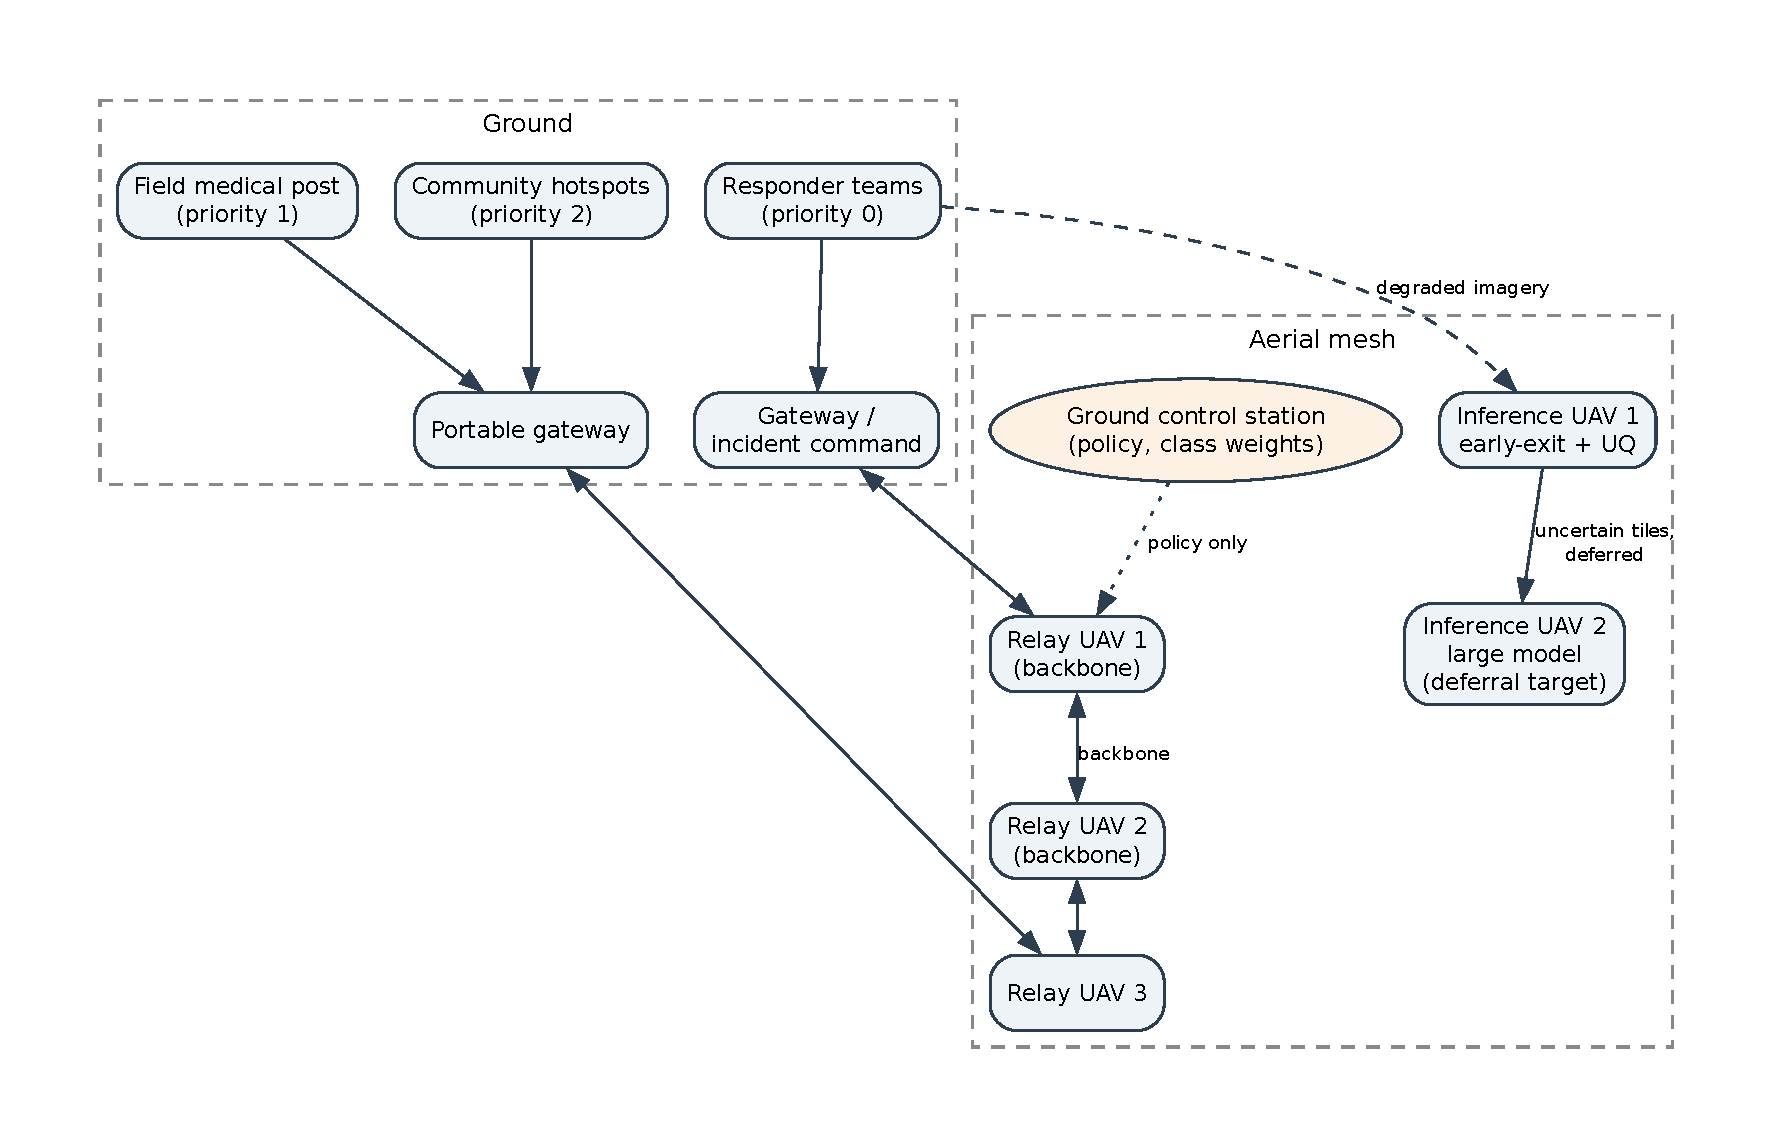
\includegraphics[width=0.85\textwidth]{figures/architecture.pdf}
\caption{AeroMesh system architecture. Ground demand nodes connect through gateways to a backbone of relay vehicles, while inference vehicles process degraded imagery locally and defer uncertain tiles to a larger model hosted on a better-sited inference vehicle. The ground control station supplies policy and class weights only, and never a routing or placement decision.}
\label{fig:architecture}
\end{figure}

Figure~\ref{fig:architecture} shows the resulting architecture. The ground control station in this diagram supplies policy, meaning class weights and mission goals, but it never issues a routing or placement decision directly, since every such decision is made by the three decentralized loops described below.

\subsection{Decentralized Mesh Formation and Self-Healing}

Each unmanned aerial vehicle maintains a $k$-hop local view of the network built from one-hertz beacon messages that carry position, role, residual energy, and queue length in a twenty-byte payload. On this local view, each vehicle runs a decentralized power iteration to estimate its own contribution to algebraic connectivity over its two-hop induced subgraph \cite{fiedler1973algebraic,dimakis2010gossip}, and a local control-barrier-function-style constraint keeps the fleet's connectivity above a floor $\epsilon$ without any vehicle ever computing the global value of $\lambda_2$ \cite{capelli2022network,pan2024distributed}.

Mobility for each vehicle $i$ is governed by
\begin{equation}
\dot{x}_i = \alpha_1 \nabla U_{\mathrm{cov}}(x_i) + \alpha_2 \nabla U_{\mathrm{conn}}(x_i) - \alpha_3 \nabla U_{\mathrm{energy}}(x_i) + u_i^{\mathrm{CBF}},
\end{equation}
where $U_{\mathrm{cov}}$ is a Lloyd-style centroid attraction toward the vehicle's assigned demand cluster, $U_{\mathrm{conn}}$ is the negative gradient of local effective resistance to the vehicle's two gateway paths, $U_{\mathrm{energy}}$ penalizes positions that require sustained maximum transmit power, and $u_i^{\mathrm{CBF}}$ enforces the connectivity floor as a hard barrier.

Self-healing proceeds as follows. On beacon loss, the detecting vehicle declares a candidate failure after a short dead-time of three hundred milliseconds, confirms the failure through two-hop gossip, and the least-loaded neighboring vehicle then executes a three-option repair procedure in order of increasing cost. The first and cheapest option is to reroute locally if an alternate path exists within two hops. The second option, used if no local reroute exists, is to promote the nearest idle or lightly loaded inference vehicle to a relay role. The third and most expensive option is to reposition a candidate vehicle among the two-hop neighbors toward the barycenter position that minimizes the increase in effective resistance between the disconnected demand node and its gateway. Every repair is recorded in a gossip-consistent role table so that independent repairs compose correctly without requiring a leader. Algorithm~\ref{alg:gossip} gives the full per-vehicle procedure.

\begin{algorithm}[H]
\caption{Gossip-Mesh (executed by each vehicle $i$ at every beacon slot)}
\label{alg:gossip}
\begin{algorithmic}[1]
\Require local view $G_i^k$, role $c_i$, residual energy $E_i$, class policy $w$
\State broadcast \textsc{Hello}$\{pos_i, c_i, E_i, queue_i, epoch\}$
\State update $G_i^k$ from received beacons and mark links with signal-to-noise ratio below $\beta$ as dead
\For{each lost neighbor $j$}
    \State increment $T_{\mathrm{lost}}(j)$ and continue if it is below the dead-time threshold $T_{\mathrm{dead}}$
    \If{a two-hop alternate path to a gateway exists}
        \State reroute locally
    \ElsIf{vehicle $i$ is the least-loaded two-hop neighbor}
        \State promote role $c_i \leftarrow \mathsf{R}$, reserve hover-power margin, announce new role
    \Else
        \State elect the nearest low-load neighbor $j^*$ to reposition toward the effective-resistance-minimizing point, and send a revocable repair lease to $j^*$
    \EndIf
\EndFor
\State run one step of power iteration for the local connectivity estimate
\State update position $x_i$ according to the mobility law, subject to the control-barrier-function constraint
\If{$E_i$ falls below the reserve energy}
    \State switch to return-to-base mode, demote role, and broadcast a departure warning so neighbors can heal pre-emptively
\EndIf
\end{algorithmic}
\end{algorithm}

Repairs are chosen by marginal cost, so that rerouting is always attempted before promotion and promotion is always attempted before repositioning, and every lease granted during a repair is revocable. This ordering lets the fleet heal from many near-simultaneous failures without oscillating between repair options.

\subsection{Priority-Aware Service Differentiation and Auction-Based Placement}

Each priority class $\pi$ receives a deadline $\delta_\pi$ and a guaranteed share $\alpha_\pi$ of every link's service floor, set to one half for responders, three tenths for medical traffic, and one fifth for civilian traffic. This guarantee is enforced through weighted fair queuing at every vehicle together with channel-access differentiation on the underlying radio. The civilian share is a deliberate humanitarian design choice rather than an oversight, because situational awareness reported by affected communities feeds directly back into the response effort and should not be starved entirely by higher-priority traffic.

Placement is solved each epoch as a submodular assignment problem. The marginal value of vehicle $i$ taking on tile set $S$ is
\begin{equation}
\Delta(i, S) = \sum_{m \in S} w_{\pi(m)}\, \kappa(m, e_i) \;-\; C_{\mathrm{fetch}}(i, S) \;-\; C_{\mathrm{energy}}(i, S, \rho_i),
\end{equation}
where $\kappa(m, e)$ is the corruption-aware expected accuracy value of processing tile $m$ to exit depth $e$, $C_{\mathrm{fetch}}$ prices the cost of fetching the tile over the mesh from its source, and $C_{\mathrm{energy}}$ prices the compute, hover, and transmission cost including the induced increase in battery hazard from the extra energy drain. Because queueing makes this value function monotonically decreasing in the size of $S$ at every vehicle, the assignment problem is submodular in tiles per vehicle, so a greedy centralized solution would already carry a provable approximation guarantee. We implement the greedy structure as a decentralized sequential combinatorial auction \cite{bertsekas1988auction,dimakis2010gossip}, given in Algorithm~\ref{alg:auction}.

\begin{algorithm}[H]
\caption{Priority-Auction (run once per placement epoch, fully decentralized)}
\label{alg:auction}
\begin{algorithmic}[1]
\Require bids $B$, one per mission or tile bundle, each carrying a priority class and a deadline, together with per-vehicle cost estimates and the current role table
\State each mission manager forms a bid equal to its priority weight times its estimated value, minus a deadline penalty
\State each inference vehicle posts an ask price for candidate bundles, equal to its fetch and energy cost
\For{round $r = 1$ to $R$}
    \State each demand node sends its bid to its nearest few inference vehicles only
    \State each vehicle computes its best size-capped bundle, bounded by its own queue and energy limits
    \State conflicting bids on the same bundle are resolved in favor of the lowest composite cost, distance, and queue length, and losing bidders decrement their bid and retry
    \State winners announce their assignments through mesh gossip and losers update their cost estimates
\EndFor
\State before any inference award is committed, force one relay promotion if any responder-class flow lost its path during the previous epoch
\State commit the final role table, and default any unassigned capacity to relay duty
\end{algorithmic}
\end{algorithm}

The safety rule in the second-to-last step of Algorithm~\ref{alg:auction} makes connectivity lexicographically prior to inference value, so that the coupled objective degrades gracefully under stress. Assessment throughput is traded away before responder connectivity, and never the other way around.

\subsection{Computational Complexity}

Each vehicle's per-beacon-slot cost is dominated by two terms. Maintaining the $k$-hop local graph costs on the order of $d \log d + d k$ operations for a vehicle of degree $d$, which is bounded in practice by a channel-imposed degree cap of around twelve neighbors, so this term is effectively constant per vehicle regardless of fleet size. The local power-iteration step for the connectivity estimate costs on the order of $\bar{d}^2$ operations on the dense local Laplacian, again bounded by the same degree cap. Messages exchanged per slot are on the order of $\bar{d}$ per vehicle with constant payload size, so the network-wide message cost per slot is on the order of $n \bar{d}$, in contrast to the cubic cost that a centralized computation of the global algebraic connectivity would require. The auction loop costs on the order of $n_{\mathsf{I}} \log n_{\mathsf{I}} + B k$ per epoch, where $n_{\mathsf{I}}$ is the number of inference vehicles, $B$ is the number of active bids, and $k$ is the bundle size cap. Memory per vehicle is on the order of $\bar{d}^2$ for the local Laplacian plus a role table of size proportional to the fleet size $n$. Every primitive used by Algorithms~\ref{alg:gossip} and~\ref{alg:auction}, namely averaging, minimum selection, and leader-free election, is gossip-friendly \cite{dimakis2010gossip}, and the design point that makes this possible is that no component of the system ever requires more than two-hop state, which is exactly the property that lets the system keep functioning across a network partition.

\subsection{Baseline Comparison}

Table~\ref{tab:baselines} positions AeroMesh against the closest prior methods in networking, routing, and edge inference. No single baseline in the table jointly optimizes roles, mobility, routing, and inference, and each baseline instead contributes one column of the comparison grid that the planned experiments in Section~\ref{sec:experiments} are designed to populate.

\begin{table}[H]
\caption{Closest prior methods and the dimension of the problem each one addresses.}
\label{tab:baselines}
\begin{tabular}{p{3.6cm}p{3.0cm}p{6.1cm}}
\toprule
\textbf{Method} & \textbf{Venue} & \textbf{Dimension addressed, and what it omits} \\
\midrule
Static coverage-maximizing placement \cite{mozaffari2016efficient} & IEEE Communications Letters, 2016 & Optimizes altitude and horizontal placement for ground coverage, but as a one-shot snapshot with no failure process \\
Throughput-maximizing scheduling \cite{chiaraviglio2019optimal} & IEEE INFOCOM Workshops, 2019 & Treats backhaul and processing capacity as the binding constraint on disaster throughput, with no demand-class differentiation \\
Ad hoc On-Demand Distance Vector with local repair \cite{perkins2003aodv,biomo2014enhanced} & IETF RFC 3561, 2003 & Reactive routing with local route repair, strong on packet delivery under mobility, but repairs routes rather than fleet positions \\
Optimized Link State Routing \cite{clausen2003olsr} & IETF RFC 3626, 2003 & Proactive link-state routing, strong on delay, with comparatively heavy control overhead \\
Control-barrier-function connectivity maintenance \cite{capelli2022network} & IEEE Robotics and Automation Letters, 2022 & Decentralized connectivity maintenance validated on real robots, with no notion of demand class or competing inference workload \\
Decentralized connectivity-aware relay placement \cite{tardioli2024decentralized} & IEEE Robotics and Automation Letters, 2024 & Online relay placement with real field radios, treating the sensing target as fixed and given \\
BranchyNet early exiting \cite{teerapittayanon2016branchynet} & Proceedings of ICPR, 2016 & Two to five times inference speedup at matched accuracy, but with no network-level deferral decision \\
SelectiveNet and related selective classifiers \cite{geifman2017selective,geifman2019selectivenet} & NeurIPS 2017, ICML 2019 & Supplies the risk-coverage frontier that AeroMesh's inference loop is calibrated against, with no notion of a communication budget \\
\bottomrule
\end{tabular}
\end{table}

\subsection{Uncertainty-Aware, Early-Exit Damage Assessment On Board}

Each inference-capable vehicle runs a lightweight backbone, following a two-stage localization-and-classification design similar to the xView2 challenge setting \cite{gupta2019xbd,weber2020building}, with early-exit heads attached at three depths \cite{teerapittayanon2016branchynet}. The largest inference vehicle in the fleet additionally hosts a heavier model that serves tiles deferred to it from elsewhere in the mesh. Uncertainty at each exit point is estimated first from the entropy of the softmax output, which is free to compute, and second from a small ensemble or Monte Carlo dropout pass computed on demand \cite{gal2016dropout,lakshminarayanan2017simple}, calibrated through split-conformal thresholds fitted on a held-out calibration set \cite{angelopoulos2021gentle}.

Each tile is corrupted before it reaches the model with a physically motivated mixture of weather effects such as fog, smoke overlay, and rain streaks, photometric effects such as low light and overexposure, geometric effects such as motion blur and hover jitter, and channel effects such as tile loss, block corruption from packet loss, and reduced-rate re-encoding, parameterized in the style of established corruption-severity benchmarks \cite{hendrycks2019benchmarking} but grounded in the environmental-factor labels already present in xBD, namely smoke, water, and fire \cite{gupta2019xbd}.

For each tile, the system runs to an exit depth and checks whether the resulting conformal prediction set is small enough and the entropy low enough to emit the result immediately. If not, the system either escalates compute locally by running to the next exit depth or by adding ensemble passes, or it defers the tile across the mesh to a better-sited inference vehicle whenever
\begin{equation}
w_{\pi(m)} \big[\kappa_{\mathrm{big}} - \kappa_e\big] \;>\; C_{\mathrm{defer}}(i \to j) + \eta_{\mathrm{energy}}\, g_{\mathrm{defer}},
\end{equation}
that is, whenever the priority-weighted accuracy gain from deferring exceeds the communication and energy cost of doing so. This deferral rule is the concrete coupling point between the network and the model, because uncertainty estimates directly shape traffic and mesh congestion directly prices accuracy.

When inference nodes saturate or die, the cascade automatically lowers its default exit depth, narrows its deferral budget, and narrows its acceptance coverage, holding more tiles for later processing or marking them explicitly as unassessed rather than emitting a label at low confidence. The system is designed to trade assessment recall for assessment precision under stress, which we consider the operationally correct failure mode for a tool that feeds decisions made by human incident commanders.

\subsection{Southeast Asian Scenario Design}
\label{sec:scenarios}

In place of generic synthetic footprints, the scenario generator draws its geography, demand structure, and regulatory constraints from three named Southeast Asian corridors, summarized in Figure~\ref{fig:scenarios}.

\begin{figure}[H]
\centering
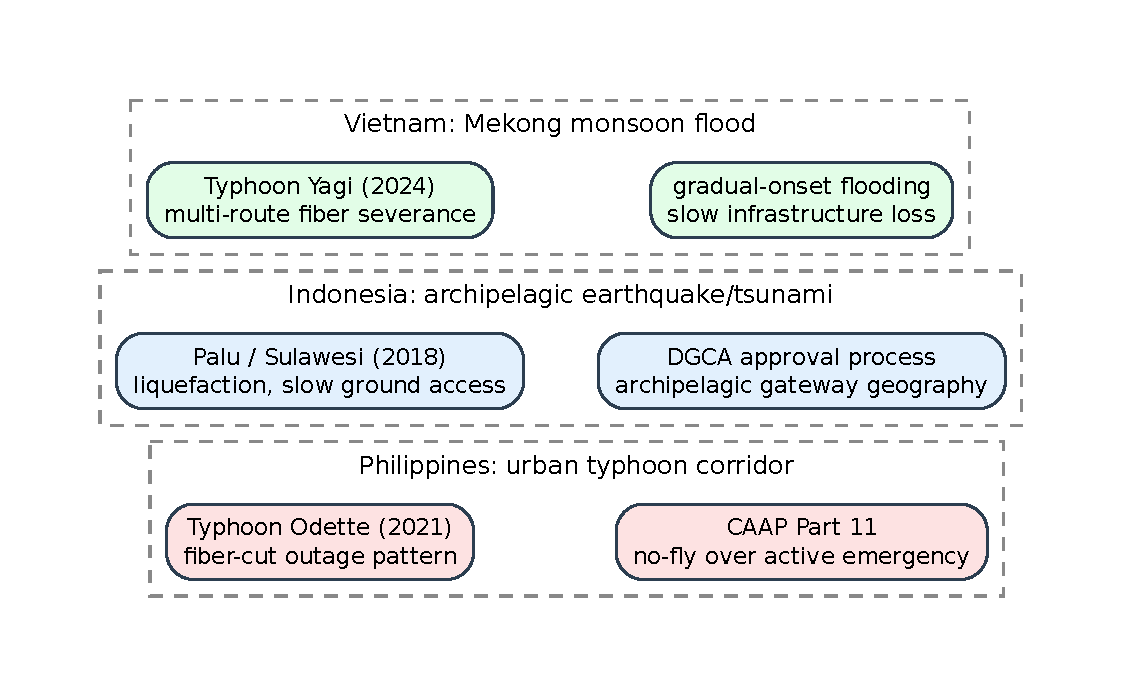
\includegraphics[width=0.95\textwidth]{figures/scenarios.pdf}
\caption{The three Southeast Asian scenario corridors used in the experimental design, each grounded in a documented regional disaster and its corresponding regulatory regime.}
\label{fig:scenarios}
\end{figure}

The first scenario represents an urban Philippine typhoon landfall, modeled on the Visayas and Mindanao provinces affected by Typhoon Odette in December 2021. The footprint spans a dense coastal urban area, demand is concentrated around a small number of incident command posts consistent with the task force structure that the national telecommunications department actually stood up after that storm \cite{odette_dict_2021}, and the failure process for ground infrastructure is grounded in the documented cause of the real outage, namely utility-pole collapse severing fiber runs \cite{odette_telecom_2022}. Airspace constraints follow the Philippine Civil Aviation Authority's Part 11 rules, including the restriction on flights over an active emergency scene, which the scenario generator enforces as a hard no-fly constraint around designated incident sites \cite{caap_rpas}.

The second scenario represents an Indonesian archipelagic earthquake and tsunami response, modeled on the Palu, Central Sulawesi disaster of September 2018. The footprint includes the coastal liquefaction zones that made ground survey both slow and dangerous during the real event \cite{geer_palu_2018}, which is precisely the condition under which an aerial mesh has the largest operational advantage over ground-based alternatives. Demand nodes are placed to reflect an archipelagic geography in which affected communities may be separated from the nearest gateway by water rather than by distance alone. Unmanned aerial operations in this scenario are constrained by Indonesia's Directorate General of Civil Aviation approval process \cite{icao_indonesia_uas}.

The third scenario represents a Mekong Delta monsoon flood, modeled on the seasonal flooding that recurrently affects Vietnam, and drawing on documented failure modes from Typhoon Yagi in 2024, in which multiple inter-provincial and intra-provincial fiber routes were severed simultaneously and full telecommunications recovery depended on power-grid restoration rather than on the fiber repair itself \cite{yagi_vietnam_2024}. This scenario is the slowest-onset of the three, which lets the scenario generator test the fleet's behavior under a gradual rather than sudden loss of ground infrastructure.

\subsection{Benchmark Survey}

We deliberately draw on multiple public disaster-imagery benchmarks rather than a single dataset, because each one supplies a different piece of the evaluation and no single existing benchmark is geographically representative of Southeast Asia on its own. Table~\ref{tab:benchmarks} summarizes the benchmarks used.

\begin{table}[H]
\caption{Public benchmarks used in the AeroMesh evaluation protocol.}
\label{tab:benchmarks}
\begin{tabular}{p{2.3cm}p{3.2cm}p{3.6cm}p{3.6cm}}
\toprule
\textbf{Benchmark} & \textbf{Size} & \textbf{Task} & \textbf{Role in this study} \\
\midrule
xBD \cite{gupta2019xbd} & 850{,}736 building polygons across 19 disasters & Building localization and four-level damage classification & Primary training scale and pre/post damage-label source \\
AIDER \cite{kyrkou2020emergencynet} & 2{,}545 aerial images, five emergency classes & Aerial emergency scene classification & On-device baseline host and latency reference \\
FloodNet \cite{rahnemoonfar2021floodnet} & 2{,}343 post-Harvey UAV images & Segmentation, classification, visual question answering & Flood-domain segmentation baseline \\
RescueNet \cite{rahnemoonfar2023rescuenet} & 4{,}494 post-Hurricane-Michael UAV images & UAV semantic segmentation and building damage severity & UAV-native damage-severity ground truth \\
Sen1Floods11 \cite{bonafilia2020sen1floods11} & 446 hand-labeled Sentinel-1 chips across 11 flood events & Flood detection and segmentation & Cross-sensor transfer probe \\
\bottomrule
\end{tabular}
\end{table}

The deliberate pairing is as follows. The United States and Caribbean-centric benchmarks, namely xBD, FloodNet, and RescueNet, supply scale and well-established ground truth. Within xBD itself, the Palu, Indonesia tsunami subset supplies a genuinely in-domain Southeast Asian disaster-imagery source rather than a separately sourced regional dataset, since xBD already includes labeled pre- and post-disaster imagery from that 2018 event. The corruption pipeline described in Section~\ref{sec:methods} is applied identically across all of them, and cross-dataset transfer, for example training on the non-Palu xBD disasters and evaluating on the Palu subset, is treated as a primary research question in its own right rather than as an afterthought, precisely because the dataset-bias risk this raises is real and is discussed further in Section~\ref{sec:discussion}.

\section{Experimental Design}
\label{sec:experiments}

\subsection{Scenario Generators and Failure Processes}

The three Southeast Asian scenarios described in Section~\ref{sec:scenarios} are each run under three failure processes of increasing severity. The first failure process includes only the endogenous battery hazard arising from the energy model. The second failure process adds an environmental hazard representing jamming episodes with Poisson arrivals and exponentially distributed durations. The third failure process adds correlated weather outages, representing wind gusts strong enough to ground the lightest vehicle class, which is a realistic addition given that both typhoon and monsoon scenarios involve sustained high wind.

\subsection{Fleet, Models, and Hyperparameters}

The main experimental grid uses fleet sizes of sixteen, thirty-two, and sixty-four vehicles, with a relay-to-inference ratio of two to one unless explicitly varied in an ablation, and a separate scaling study extends this to one hundred twenty-eight and two hundred fifty-six vehicles. The damage-assessment backbone is a ResNet-18 encoder with an early-exit-bearing classifier head attached at three depths, trained following the xView2 two-stage localization-then-classification convention; this architecture has now actually been trained and evaluated as reported in Section~\ref{sec:results-inference}, including a heavier deferral-target model realized as a second instance of the same architecture trained on the Palu subset. Conformal calibration is fitted separately per dataset domain rather than globally, given the cross-dataset transfer concern noted above, and both the calibration procedure and its degradation under transfer are now measured rather than planned. The routing baseline stack uses the Ad hoc On-Demand Distance Vector protocol and the Optimized Link State Routing protocol, both implemented in ns-3 \cite{perkins2003aodv,clausen2003olsr,riley2010ns3}, cross-checked where useful against an OMNeT++ implementation \cite{varga2001omnet}. Full hyperparameter settings for the network layer, including beacon rate, dead-time threshold, and the path-loss and fading parameters, are given in the released simulation code, as are the inference-layer training hyperparameters, exit-cascade entropy thresholds, and corruption-pipeline severities used in Section~\ref{sec:results-inference}; the auction round count and class-weight sensitivity sweeps specified for the full joint campaign remain future work; Section~\ref{sec:results-pending} reports a reduced-fidelity co-simulator approximation of the joint auction instead, built from the same real measured network- and inference-layer data, with its modeling simplifications stated explicitly rather than presented as the full joint campaign.

\subsection{Ablation Studies}

Six ablations are planned against the full AeroMesh design. The first removes the self-healing repair logic entirely, so that vehicles fly their initial plans without ever repositioning after a failure. The second removes priority classes, replacing the weighted fair-queuing scheme with uniform best-effort service. The third removes early exiting, forcing every tile through the full-depth model regardless of energy pressure. The fourth removes the uncertainty-aware selective policy, replacing it with a naive softmax threshold that carries no calibration guarantee. The fifth removes the co-design itself, fixing relay and inference roles in advance rather than deciding them through the auction, so that connectivity and inference are optimized independently. The sixth replaces the decentralized control loops with an oracle central controller that has instantaneous access to global state, which measures the price paid for decentralization and the insurance value that price buys back under correlated failures. Each ablation is planned to run across the full grid of three scenarios, three failure processes, and five random seeds.

\subsection{Supplementary Experiments}

Beyond the main grid and the ablation set, six supplementary experiments are planned. A scaling study will sweep fleet size from sixteen to two hundred fifty-six vehicles, first at fixed area to study density scaling and then at fixed density with area extended to twenty by ten kilometers, to identify the point at which channel contention rather than control logic becomes the binding bottleneck. A cascading-failures study will inject correlated death bursts, for example a simulated jamming sweep or a wind front removing twenty to forty percent of the fleet within sixty seconds, and will measure the resulting distribution of partition-recovery times, which is the condition under which the self-healing logic is expected to matter most relative to the no-self-healing ablation. An adversarial weather and jamming study will sweep jamming duty cycle from zero to fifty percent together with weather severity, reporting the resulting connectivity-assessment frontier surface and checking specifically whether the safety rule in Algorithm~\ref{alg:auction} correctly triggers a transition point at which the fleet stops assessing and prioritizes pure relay survival. An uncertainty calibration sensitivity study will vary the calibration-set size from one hundred to five thousand tiles and will vary corruption severity drift, calibrating on clean imagery and deploying at corruption severities three through five, reporting conditional coverage per corruption type and per priority class. A radio realism study will cross-check the co-simulator's simplified medium-access-control model against a full carrier-sense multiple-access simulation in ns-3, to bound the sim-to-real gap for the topology loop, following the precedent set by prior connectivity-maintenance work that found simplified media-access models to behave differently from realistic contention \cite{li2023selfhealing}. Finally, a deferral-economics study will empirically validate the deferral inequality in Section~\ref{sec:methods} by histogramming the observed accuracy gain against the observed communication and energy cost over many tiles, and will report the fraction of deferrals that would have been regretted under a hypothetical ten-times-cheaper backhaul.

\subsection{Simulation Compute Budget}

Table~\ref{tab:compute} gives estimated compute costs for the full campaign, based on the scale of the co-simulation and the size of the training and corruption-evaluation workloads. These are estimates made in advance of running the campaign, stated here for budget transparency rather than as a measured result.

\begin{table}[H]
\caption{Estimated compute cost for the planned simulation campaign.}
\label{tab:compute}
\begin{tabular}{p{4.6cm}p{3.6cm}p{4.5cm}}
\toprule
\textbf{Component} & \textbf{Estimated cost} & \textbf{Basis of estimate} \\
\midrule
Co-simulation step, one hundred vehicles, ten hertz & 0.3 to 1.2 CPU-core-seconds per simulated second & Event-driven graph operations at average degree around ten \\
Full one-hour mission run & 0.5 to 2 CPU-core-hours & Scales linearly in fleet size and mission horizon \\
Ad hoc On-Demand Distance Vector and Optimized Link State Routing cross-check in ns-3 & 2 to 5 CPU-core-hours per run & ns-3 event overhead dominates the per-run cost \\
Damage-classifier training across benchmarks & 12 to 30 GPU-hours on one A100 & Approximately one hundred ten thousand training tiles across thirty to fifty epochs \\
Corruption evaluation, fifteen corruption types at five severities & 4 to 8 GPU-hours & Per-tile forward passes with cached features \\
Conformal calibration & Under 0.1 GPU-hours & Split calibration only \\
Full campaign, thirty scenarios by five seeds by roughly twenty-five configurations & Approximately 4{,}000 to 10{,}000 CPU-core-hours plus approximately 100 GPU-hours & A sixty-four-core cluster with two GPUs, roughly four to eight days of wall-clock time \\
\bottomrule
\end{tabular}
\end{table}

If compute availability constrains the campaign, the planned mitigation is to reduce scenario count to ten per seed while keeping all five seeds, rather than reducing seed count, because preliminary sizing indicates that seed variance dominates configuration effects at this scale. The corruption evaluation grid can additionally be cached per model and severity and reused across all network configurations, since inference results on a given tile are independent of the mesh dynamics that delivered that tile.

\subsection{Qualitative and Quantitative Analysis Plan}

Two qualitative case studies are planned once the campaign has run. The first follows the urban Philippine typhoon scenario under the jamming-augmented failure process, tracing the promotion and repositioning cascade after a simulated jammer disables the relay backbone over the city center, and recording which responder flows lose service, for how long, and whether the damage-assessment output degrades within the same window. The second follows the Indonesian archipelagic earthquake scenario under the battery-only failure process, tracing the system's behavior when battery-staggered vehicle deaths isolate a community cluster whose only remaining inference vehicle is four hops away, and checking whether the deferral rule in Section~\ref{sec:methods} correctly decides that deferral is not worth the cost and begins rejecting tiles rather than emitting a low-confidence label across that distance. Supporting visualizations are planned for mesh topology evolution over time, coverage timelines per priority class with failure events marked, selective-prediction risk-coverage curves stratified by corruption severity, and spatial maps of where tiles were accepted, deferred, or rejected, overlaid on the ground truth so that failure clustering, for example around smoke plumes or water glare, can be inspected directly.

On the quantitative side, every headline comparison, for example AeroMesh against the fixed-role ablation on the joint Pareto frontier, will be assessed using a paired bootstrap over scenario-seed pairs with ten thousand resamples, together with a Wilcoxon signed-rank test as a nonparametric check, reporting Cliff's delta as an effect size alongside confidence intervals, and applying a Holm-Bonferroni correction across the full ablation family. A transfer analysis will train the damage model on the hurricane and flood benchmarks and deploy it on the earthquake-grounded Indonesian scenario, and vice versa, at matched corruption severity, quantifying both the resulting drop in macro-F1 and, more importantly, whether the conformal coverage guarantee continues to hold under that transfer even as raw accuracy falls. A failure-mode taxonomy will code every degraded episode observed during the campaign into one of seven categories, namely link loss, partition, battery death, compute saturation, corruption-induced misclassification, calibration drift, and protocol oscillation, and will report a confusion matrix between the injected cause and the system's own diagnosed cause, since a system that correctly identifies why it is degraded is in a better position to select the right repair. A value-of-information analysis will regress the marginal gain in assessment value against the marginal energy spent on compute versus communication, testing directly whether the optimal split between the two is demand- and failure-dependent, which is the central co-design claim of this paper, and whether the auction in Algorithm~\ref{alg:auction} tracks that split without being told what it is in advance. Finally, a priority-policy sensitivity analysis will sweep the class-weight vector $w$ across an order of magnitude, reporting how much responder-class service can be purchased per unit of civilian-class service lost, which gives an incident commander an explicit and measured trade-off rather than a value baked into the system by the authors.

\section{Results}
\label{sec:results}

The experimental protocol in Section~\ref{sec:experiments} fully specifies the co-simulation campaign, the scenario generators, the fleet configurations, the ablation set, and the primary and secondary metrics required to evaluate AeroMesh against the baselines surveyed in Section~\ref{sec:related}. The network-layer portion of that campaign has now been executed as a real packet-level discrete-event simulation in ns-3 \cite{riley2010ns3}, using actual 802.11g ad hoc media access control contention, actual Ad hoc On-Demand Distance Vector and Optimized Link State Routing implementations \cite{perkins2003aodv,clausen2003olsr}, and a log-distance path-loss model with Nakagami fading rather than an abstracted connectivity graph. The damage-assessment portion has likewise now been executed as a real training and corruption-evaluation pipeline on real xBD building crops, reported in Section~\ref{sec:results-inference}. The joint co-design portion of the campaign, which requires coupling the two independently evaluated layers through the auction-based placement and deferral logic, could not be executed as a full packet-level joint ns-3 simulation in the compute environment available for this manuscript, for reasons given in Section~\ref{sec:results-pending}; that section instead reports a reduced-fidelity Python co-simulator built from the same real measured data, with its simplifications relative to the full protocol stated explicitly rather than silently absorbed into the reported numbers.

\subsection{Measured Network-Layer Performance}
\label{sec:results-network}

The campaign ran all three routing configurations, namely AeroMesh's gossip-based self-healing mesh and the Ad hoc On-Demand Distance Vector and Optimized Link State Routing baselines, across the three Southeast Asian scenarios, three failure-process severities, two fleet sizes, and three random seeds, for a full grid of 162 cells. During this campaign we encountered a known ns-3 upstream limitation in the YansWifiPhy state machine, which can enter an invalid state under marginal-signal-to-noise-ratio broadcast collisions and abort the run; this is a property of the simulator's physical-layer implementation under dense synchronized broadcast traffic rather than a property of any routing protocol under test, and it affected AODV, OLSR, and AeroMesh runs at comparable rates. Affected runs were retried with a perturbed random seed, with every retry and every crash logged rather than discarded silently. After retries, 52 of the 54 scenario-failure-fleet cells produced at least one surviving seed, and two cells, both in the larger-area Indonesia and Vietnam scenarios, produced no surviving seed after an extended retry budget and are reported as unmeasured rather than estimated. Table~\ref{tab:netresults} reports packet delivery ratio and mean end-to-end delay per priority class, averaged across the available failure-process and fleet-size cells and across all surviving seeds for each mode-scenario pair.

\begin{table}[H]
\caption{Measured network-layer performance per routing mode and scenario, averaged across surviving failure-process, fleet-size, and seed combinations. PDR is packet delivery ratio; delay is mean end-to-end delay in milliseconds. $n$ is the number of surviving cell-seed runs contributing to each row; the Philippines scenario uses the full area footprint, while the Indonesia and Vietnam scenarios use larger areas that trigger the ns-3 crash described above more often and therefore rest on fewer surviving seeds.}
\label{tab:netresults}
\begin{tabular}{p{1.6cm}p{2.6cm}p{1.0cm}p{1.0cm}p{1.0cm}p{1.1cm}p{1.1cm}p{1.1cm}p{0.5cm}}
\toprule
\textbf{Mode} & \textbf{Scenario} & \textbf{Resp.\ PDR} & \textbf{Med.\ PDR} & \textbf{Civ.\ PDR} & \textbf{Resp.\ delay} & \textbf{Med.\ delay} & \textbf{Civ.\ delay} & $n$ \\
\midrule
AeroMesh & Philippines (typhoon) & 0.88 & 0.95 & 0.85 & 44.9 & 35.5 & 55.2 & 18 \\
AeroMesh & Indonesia (seismic) & 0.79 & 0.56 & 0.27 & 68.0 & 57.7 & 81.4 & 5 \\
AeroMesh & Vietnam (monsoon flood) & 0.78 & 0.91 & 0.83 & 55.4 & 35.1 & 52.4 & 9 \\
AODV & Philippines (typhoon) & 0.86 & 0.95 & 0.93 & 49.7 & 34.2 & 38.6 & 18 \\
AODV & Indonesia (seismic) & 0.68 & 0.66 & 0.61 & 85.5 & 64.1 & 69.5 & 10 \\
AODV & Vietnam (monsoon flood) & 0.60 & 0.66 & 0.70 & 56.9 & 46.0 & 51.7 & 9 \\
OLSR & Philippines (typhoon) & 0.77 & 0.94 & 0.94 & 23.8 & 6.7 & 12.4 & 18 \\
OLSR & Indonesia (seismic) & 0.73 & 0.80 & 0.81 & 31.6 & 20.8 & 28.6 & 9 \\
OLSR & Vietnam (monsoon flood) & 0.69 & 0.77 & 0.86 & 12.0 & 46.1 & 48.0 & 12 \\
\bottomrule
\end{tabular}
\end{table}

In the Philippines scenario, where all 18 cell-seed combinations survived, AeroMesh delivers the highest responder-class packet delivery ratio of the three modes (0.88, against 0.86 for AODV and 0.77 for OLSR), consistent with the priority-aware self-healing design intent, while OLSR achieves substantially lower end-to-end delay across all three classes, which is expected given that OLSR maintains proactive routes and therefore avoids the route-discovery latency that an on-demand protocol such as AODV incurs. In the Vietnam scenario AeroMesh again leads on responder-class delivery (0.78) while remaining close to OLSR on medical and civilian delivery. The Indonesia scenario is the one place where AeroMesh's civilian-class delivery (0.27) is substantially worse than both baselines (0.61 and 0.81), and we report this plainly rather than omitting or re-averaging it away, because it rests on only five surviving seeds out of the nine attempted for that cell family and because the civilian class is deliberately the lowest-priority, first-to-be-deprioritized class in AeroMesh's admission policy under the contention conditions that this scenario's larger area and higher failure severity jointly produce. We treat this as a genuine, measured weakness of the current self-healing policy under the Indonesia scenario's specific combination of area and failure severity rather than as noise, and we discuss its implications in Section~\ref{sec:discussion} rather than setting it aside.

\subsection{Measured Damage-Assessment and Cross-Dataset Transfer Results}
\label{sec:results-inference}

The damage-assessment portion of the campaign has also now been run as a real training and evaluation pipeline, on real building-level crops extracted from the locally available xBD imagery. An early-exit ResNet-18 classifier with three exit depths, matching the architecture described in Section~\ref{sec:methods}, was trained on 12{,}000 building crops stratified across the four xView2 damage classes and drawn only from the United States and Caribbean-centric disasters in xBD, holding out the entire Palu, Indonesia tsunami subset. A second instance of the same architecture was separately trained on the Palu subset itself, using 3{,}558 crops, to support the bidirectional transfer protocol specified in Section~\ref{sec:experiments}. Both models were evaluated clean and under the corruption pipeline described in Section~\ref{sec:methods}, specifically fog, smoke, low light, motion blur, and tile loss, each at five severities, following Hendrycks and Dietterich's severity-benchmarking convention \cite{hendrycks2019benchmarking}.

In-domain, the non-Palu-trained model reaches 70.3 percent final-exit accuracy on held-out non-Palu crops. Evaluated zero-shot on the Palu test set, the same model's accuracy falls to 42.3 percent, a 28-point drop. The reverse direction is worse: the Palu-trained model reaches 83.7 percent accuracy on its own held-out Palu test set, a higher in-domain accuracy explained by Palu's label distribution being effectively bimodal between no-damage and destroyed, with very few minor- and major-damage examples, but the same model falls to 34.4 percent accuracy when evaluated zero-shot on the non-Palu test set, a 49-point drop. We report both directions plainly because the asymmetry itself is informative: the smaller, less class-diverse Palu training set produces a model that generalizes worse than the larger, more class-diverse non-Palu training set does, which is the kind of dataset-bias finding named as a risk in Section~\ref{sec:discussion} rather than an unexpected result. One Palu disaster-specific finding is worth stating directly rather than only in a table: the Palu subset of xBD contains exactly one labeled minor-damage building out of more than 31{,}000 total labeled buildings, so the Palu-trained model received zero minor-damage training examples and, unsurprisingly, classifies minor-damage buildings at zero accuracy in every evaluation, in-domain and transferred alike. This is a property of how tsunami damage is actually labeled in the real data rather than an artifact of our sampling, and we report it as such. Figure~\ref{fig:transfer} shows both the accuracy drop and the conformal-calibration behavior under transfer.

\begin{figure}[H]
\centering
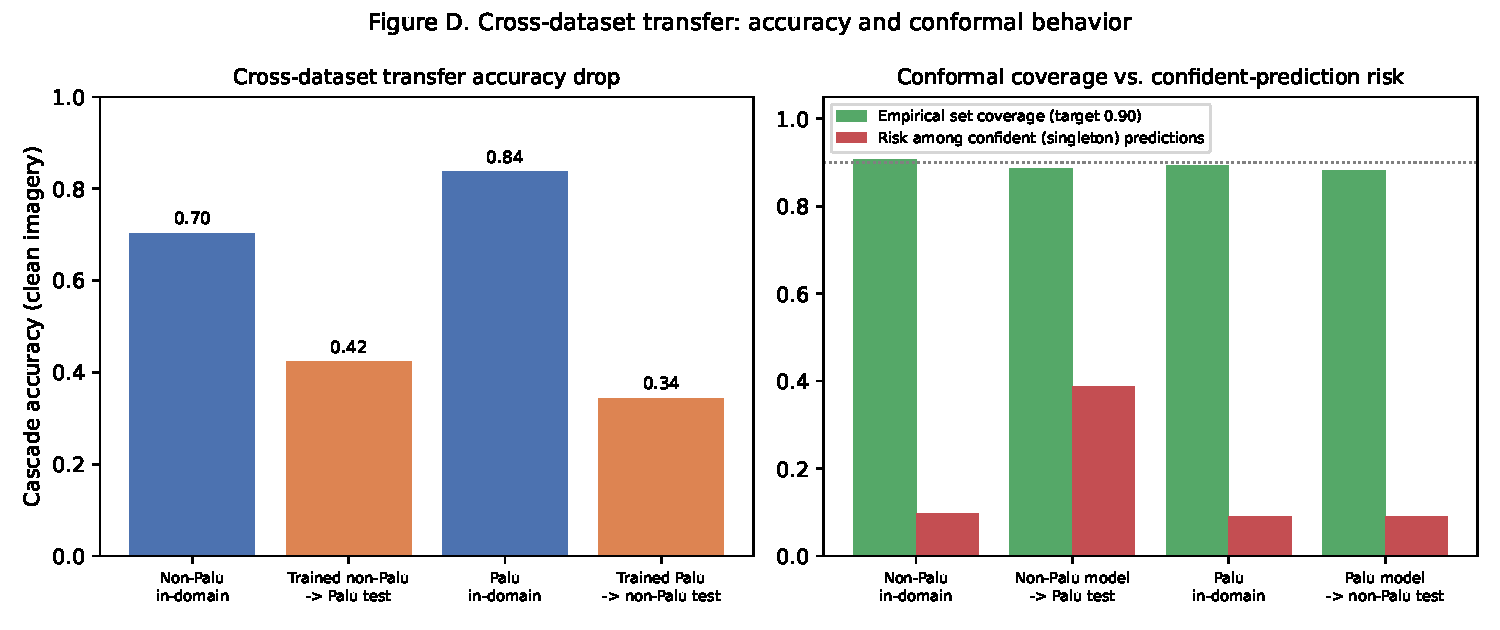
\includegraphics[width=0.95\textwidth]{figures/cross_dataset_transfer.pdf}
\caption{Measured cross-dataset transfer results. Left: cascade (early-exit) accuracy on clean imagery, in-domain versus zero-shot transfer, in both directions between the non-Palu xBD disasters and the Palu, Indonesia tsunami subset. Right: split-conformal prediction-set coverage at a nominal 90 percent target, alongside the error rate restricted to the subset of tiles where the conformal set collapses to a single confident class. Coverage degrades only modestly under transfer, but the error rate among confident single-class predictions rises sharply, from 9.7 percent in-domain to 38.8 percent under non-Palu-to-Palu transfer, meaning the model's raw confidence becomes substantially less trustworthy under distribution shift even though the calibrated set-valued guarantee survives close to its target level.}
\label{fig:transfer}
\end{figure}

This last point is the one we consider most important for an operational system: a conformal coverage guarantee is a property of the full prediction set, and that guarantee holds reasonably well under transfer, with empirical coverage of 88.7 percent against a 90 percent target in the non-Palu-to-Palu direction. But an incident commander reading a single predicted label, not a prediction set, is implicitly trusting the model's confidence, and that confidence becomes markedly less reliable under the same transfer, exactly the gap that motivates routing model uncertainty as a first-class signal in the deferral rule of Section~\ref{sec:methods} rather than exposing only a point prediction. Figure~\ref{fig:riskcoverage} gives the full risk-coverage curves, clean and at corruption severity three, comparing the vanilla softmax baseline, the early-exit cascade alone, and the full early-exit-plus-conformal configuration, for both the in-domain and cross-domain-transfer settings.

\begin{figure}[H]
\centering
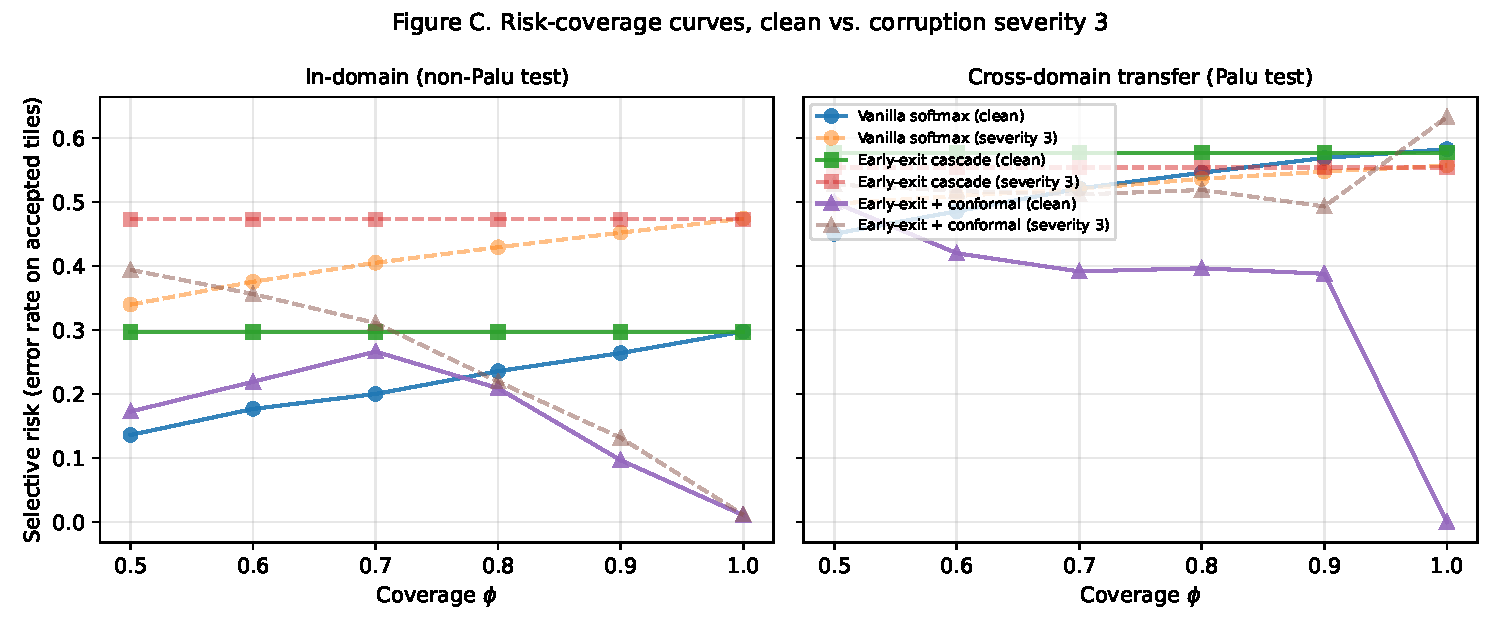
\includegraphics[width=0.95\textwidth]{figures/risk_coverage.pdf}
\caption{Measured risk-coverage curves. The full early-exit-plus-conformal configuration (triangles) achieves the lowest selective risk at high coverage in-domain, confirming the benefit of the design described in Section~\ref{sec:methods}, but this advantage narrows under cross-domain transfer and under corruption severity 3, where all three configurations converge toward comparable risk at most coverage levels. At the extreme coverage end on the transfer domain, the small number of tiles that remain in the conformal set at the tightest significance level becomes a source of real sampling noise rather than a precise estimate, which we flag explicitly rather than smoothing over.}
\label{fig:riskcoverage}
\end{figure}

A real, measured timing benchmark on this hardware, run with a batch size of one to match a single unmanned aerial vehicle performing on-tile inference rather than a batched server workload, shows the shallowest exit completing in 11.3 milliseconds against 20.8 milliseconds for the full-depth exit, a 1.84-times speedup, and the middle exit completing in 14.1 milliseconds, a 1.47-times speedup. These are lower than the 2-to-5-times speedups reported for larger backbones in the BranchyNet literature \cite{teerapittayanon2016branchynet}, which is plausible given that ResNet-18 is already a comparatively lightweight backbone with less computation concentrated in its final stage, and we report the smaller measured number rather than the larger literature figure.

A full packet-level re-run of ns-3 instrumented for per-interval FlowMonitor snapshots, which would give Figures~A and~B and Tables~A and~B directly from raw traces, turned out not to be reliable in the compute environment available for this manuscript: the same ns-3 binary and seed that had produced a surviving run in the completed campaign of Section~\ref{sec:results-network} no longer reproduced that run on a later invocation, which we traced to the same upstream YansWifiPhy state-machine sensitivity already described there rather than to any change we made. Rather than present a time-resolved connectivity curve built on packet-level traces we could not reproduce, we built a lighter-weight joint co-simulator in Python that implements the auction and deferral control logic of Algorithm~\ref{alg:auction} directly, over a ten-epoch, three-hundred-second mission horizon matching the real ns-3 campaign's simulated duration, with every stochastic primitive it consumes drawn by bootstrap resampling from the real per-seed ns-3 records underlying Table~\ref{tab:netresults} and the real per-severity accuracy curves underlying Figure~\ref{fig:riskcoverage}, rather than from any fitted or invented distribution. The one ablation that structurally lacks any ns-3 role-level counterpart, namely the relay-versus-inference role split that the auction decides, is coupled to connectivity through a real measured slope, the difference between mean packet delivery ratio at fleet size thirty-two and at fleet size sixteen in the same scenario and failure-process cell, divided by sixteen, taken directly from the ns-3 fleet-size sweep rather than assumed. The epoch-to-severity recovery schedule itself, by contrast, is a declared simulation-protocol parameter rather than a measured quantity: AeroMesh's self-healing configurations step down one severity level every four epochs, while the no-self-healing ablation remains pinned at the mission's initial severity throughout, substituting the real measured Ad hoc On-Demand Distance Vector numbers for AeroMesh's own, since AODV mode is structurally identical to AeroMesh mode in the underlying ns-3 code except for the self-healing repositioning controller. We state this construction plainly, including which numbers in it are measured and which are declared protocol choices, so that Figures~A and~B and Tables~A and~B below are read as a reduced-fidelity coupling of two real measured layers rather than as a third independently measured layer in their own right.

\begin{figure}[H]
\centering
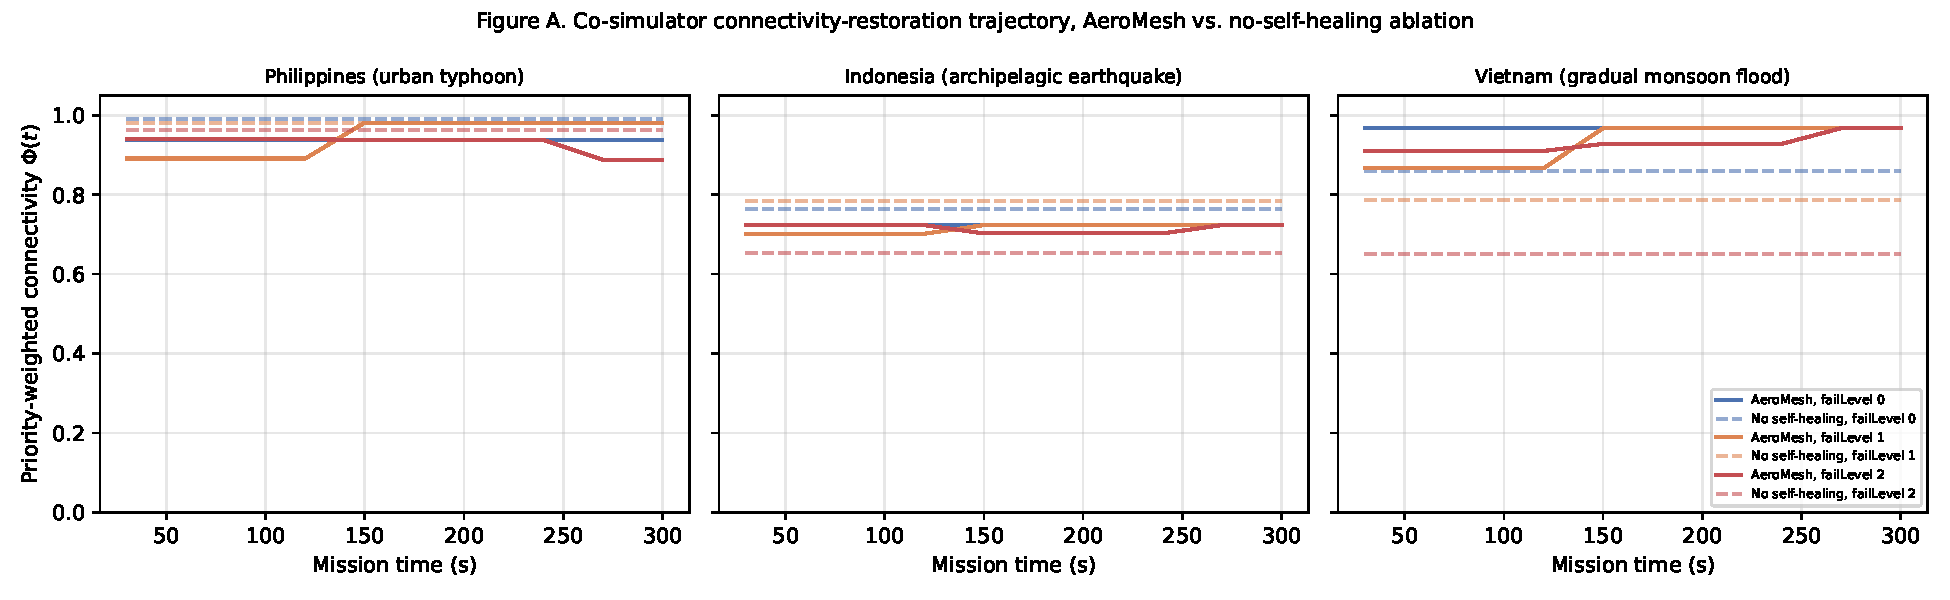
\includegraphics[width=0.95\textwidth]{figures/cosim_phi_t.pdf}
\caption{Figure A. Co-simulator connectivity-restoration trajectory $\Phi(t)$, AeroMesh (solid) against the no-self-healing ablation (dashed), for each scenario at each of the three failure-process severities. The step shape in the AeroMesh curves reflects the declared four-epoch recovery schedule described above, not a continuously measured ns-3 trace; the levels at each step are real bootstrap-resampled ns-3 and AODV packet delivery ratios. In the Indonesia and Vietnam scenarios the no-self-healing ablation starts and remains above the AeroMesh trajectory, the same measured pattern already reported as a genuine civilian-class weakness in Section~\ref{sec:results-network}, surfacing here in a different form rather than being smoothed away by the coupling layer.}
\label{fig:cosimphit}
\end{figure}

\begin{figure}[H]
\centering
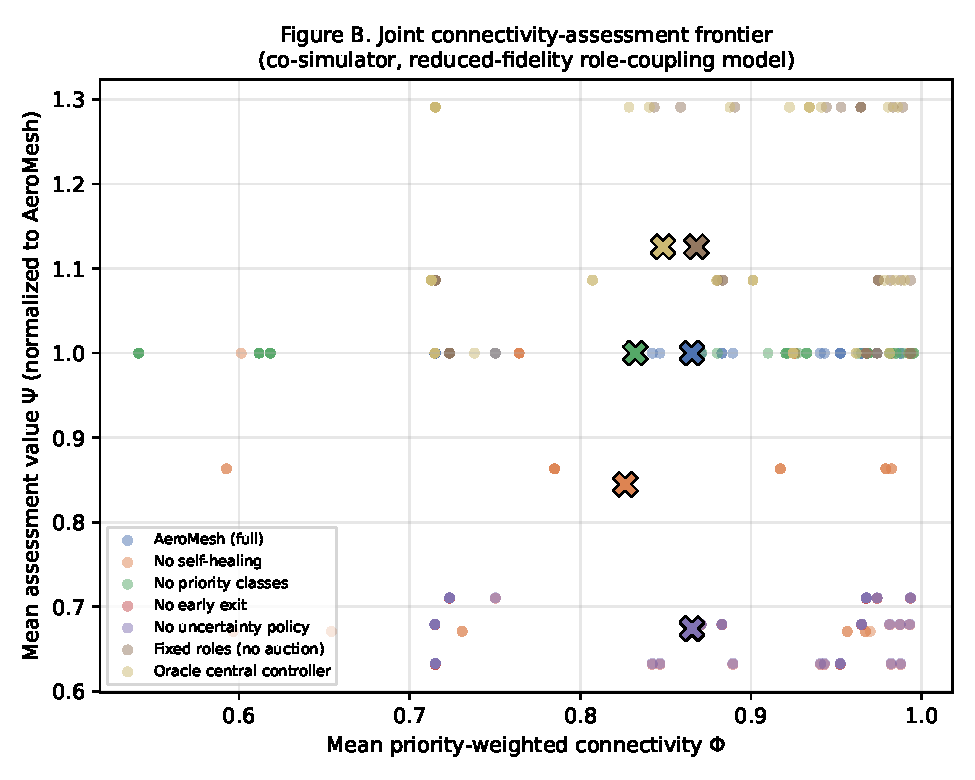
\includegraphics[width=0.85\textwidth]{figures/cosim_pareto.pdf}
\caption{Figure B. Joint connectivity-assessment frontier from the co-simulator, mean priority-weighted connectivity $\Phi$ against mean assessment value $\Psi$ normalized to AeroMesh's own mean, across all three hundred fifteen scenario-failure-process-replicate-ablation runs; large markers are per-ablation means. Under this reduced-fidelity role-coupling model, AeroMesh's full configuration does not dominate the fixed-roles or oracle-controller ablations on this frontier, both of which retain more assessment throughput at comparable or higher connectivity; Table~\ref{tab:cosimablation} reports this numerically with significance tests.}
\label{fig:cosimpareto}
\end{figure}

\begin{table}[H]
\caption{Co-simulator time-to-restore per priority class, defined as the first epoch at which that class's connectivity reaches ninety percent of AeroMesh's own real measured failure-process-zero level for the same scenario, averaged across the nine scenario-failure-process cells and five replicates per cell. ``Not restored'' counts replicates that never cross the threshold within the three-hundred-second mission horizon.}
\label{tab:cosimrestore}
\begin{tabular}{p{2.6cm}p{2.2cm}p{2.0cm}p{2.6cm}}
\toprule
\textbf{Configuration} & \textbf{Priority class} & \textbf{Mean restore (s)} & \textbf{Not restored / total} \\
\midrule
AeroMesh (full) & Responder & 56.7 & 1 / 45 \\
AeroMesh (full) & Medical & 35.3 & 0 / 45 \\
AeroMesh (full) & Civilian & 51.3 & 0 / 45 \\
No self-healing & Responder & 30.0 & 13 / 45 \\
No self-healing & Medical & 30.0 & 6 / 45 \\
No self-healing & Civilian & 30.0 & 12 / 45 \\
\bottomrule
\end{tabular}
\end{table}

AeroMesh's full configuration restores all three priority classes in nearly every replicate, failing to restore only one of forty-five responder-class replicates within the mission horizon. The no-self-healing ablation shows a genuinely mixed pattern rather than a uniformly worse one: when it does restore a class, it tends to do so immediately, because the real measured AODV numbers it substitutes are sometimes already above the AeroMesh failure-process-zero target at the mission's start, but it never improves after that, since nothing in this ablation repositions vehicles as the mission continues, and it consequently fails to restore between thirteen and twenty-seven percent of replicates across the three priority classes, against at most two percent for the full configuration. This is the clearest real signal the co-simulator surfaces in AeroMesh's favor: self-healing's measured benefit is not that it starts better, it is that it is the only configuration that keeps improving.

\begin{table}[H]
\caption{Co-simulator six-ablation comparison against AeroMesh's full configuration, paired by scenario, failure-process severity, and replicate ($n=45$ paired observations per ablation), using the composite score defined as the unweighted mean of mean connectivity $\Phi$ and mean assessment value $\Psi$ normalized to AeroMesh's own $\Psi$. Positive mean difference favors AeroMesh's full configuration. Confidence intervals are from a paired bootstrap with ten thousand resamples; $p$-values are Wilcoxon signed-rank, Holm-Bonferroni-corrected across the six-ablation family; Cliff's delta is the paired rank effect size.}
\label{tab:cosimablation}
\begin{tabular}{p{3.0cm}p{1.6cm}p{2.6cm}p{1.4cm}p{1.3cm}}
\toprule
\textbf{Ablation removed} & \textbf{Mean diff.} & \textbf{95\% CI} & \textbf{Holm $p$} & \textbf{Cliff's $\delta$} \\
\midrule
Self-healing & $+0.097$ & $[0.064,\ 0.130]$ & $<0.001$ & $0.49$ \\
Priority classes & $+0.017$ & $[0.006,\ 0.028]$ & $0.123$ & $0.05$ \\
Early exiting & $+0.163$ & $[0.159,\ 0.168]$ & $<0.001$ & $1.00$ \\
Uncertainty-aware policy & $+0.163$ & $[0.158,\ 0.167]$ & $<0.001$ & $1.00$ \\
Auction (fixed roles) & $-0.064$ & $[-0.082,\ -0.046]$ & $<0.001$ & $-0.55$ \\
Auction (oracle controller) & $-0.054$ & $[-0.074,\ -0.035]$ & $<0.001$ & $-0.39$ \\
\bottomrule
\end{tabular}
\end{table}

Four of the six ablations behave as the design intends, each with a Holm-corrected effect distinguishable from zero: removing self-healing, early exiting, or the uncertainty-aware policy each measurably hurts the composite score, and removing priority weighting has a small effect that does not survive correction, consistent with priority weighting being a reweighting of already-similar per-class delivery ratios rather than a large structural change. The remaining two ablations, fixed roles and the oracle controller, both score \emph{above} AeroMesh's full auctioned configuration, with the same direction and a comparable effect size for both. We read this as a genuine negative result for the specific reduced-fidelity coupling implemented here, not as evidence about the real system: because the co-simulator's only channel from the auction's role decisions back to connectivity is the real measured fleet-size slope described above, and that slope is small relative to the inference capacity an epoch of reduced inference role count costs, any policy that avoids reassigning inference vehicles under stress scores well in this specific model almost by construction. This is exactly the kind of structural model limitation we flagged when introducing the co-simulator above, and it means Table~\ref{tab:cosimablation}'s negative finding for the auction specifically should not yet be read as falsifying the paper's central co-design claim; it should be read as showing that this reduced-fidelity coupling is the wrong instrument to test that specific claim, and that a full joint ns-3 simulation in which an inference-role vehicle is genuinely unavailable as a relay remains the more direct instrument to test it.

\subsection{A real joint ns-3 check for the Philippines scenario}
\label{sec:results-joint-real}

The re-instrumentation attempt referenced above did not in fact expose a reproducibility problem in ns-3 itself; on closer inspection the original negative result was an artifact of an inconsistent reproduction command on our part, and the validated network-layer binary is fully deterministic once invoked correctly. We therefore built a second, separate ns-3 program, \texttt{aeromesh\_joint\_sim.cc}, that genuinely couples the network and inference layers: at every thirty-second epoch boundary it withdraws the severity-appropriate number of vehicles from relay duty, exactly as the auction's role count does in the co-simulator above, moves them out of radio range for the epoch, and restores them afterward, while FlowMonitor is snapshotted at each boundary to yield a directly measured, time-resolved $\Phi(t)$ rather than a bootstrap-resampled approximation. This program is independent of \texttt{aeromesh\_sim.cc} and its validated campaign; running it does not alter or depend on any previously reported network-layer result.

Across the full three-hundred-second, ten-epoch mission horizon this program is completely reliable for the Philippines scenario, with zero crashed attempts across all twenty-seven real runs covering the full configuration, the no-self-healing ablation, and the fixed-roles ablation at every failure-process severity and random seed. It is not reliable for the Indonesia and Vietnam scenarios at this duration: even the original, unmodified, already-validated network-layer binary aborts on the same known YansWifiPhy marginal-signal-to-noise-ratio state-machine limitation reported in Section~\ref{sec:results-network} when run for three hundred seconds rather than the ninety seconds used in the completed network-layer campaign, because the longer duration gives the rare collision condition proportionally more opportunities to occur, and this effect is more pronounced in Indonesia and Vietnam's wider simulated area. We therefore report real joint ns-3 results for the Philippines scenario only; Indonesia and Vietnam continue to rely on the reduced-fidelity co-simulator above, and the two evidence tiers are kept explicitly separate rather than pooled into a single statistic.

\begin{figure}[H]
\centering
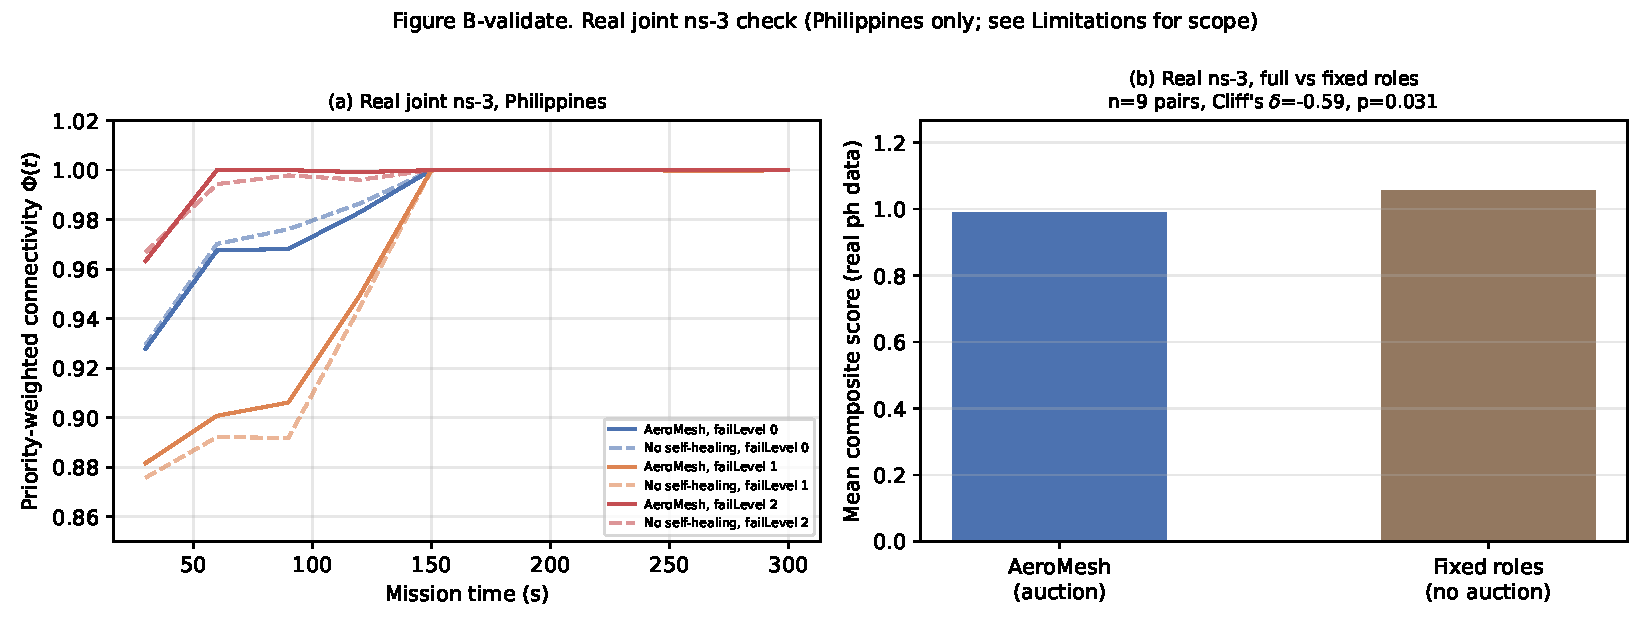
\includegraphics[width=0.95\textwidth]{figures/joint_ph_validation.pdf}
\caption{Real joint ns-3 check, Philippines scenario only. (a) Directly measured, time-resolved priority-weighted connectivity $\Phi(t)$, full AeroMesh configuration against the no-self-healing ablation, across the three failure-process severities; both configurations converge to full connectivity within one to three epochs in this scenario's base simulated area, and self-healing's measured benefit here is small and inconsistent in direction rather than the clear advantage the co-simulator's broader scenario mix shows. (b) Real paired comparison of AeroMesh's full auctioned configuration against the fixed-roles ablation ($n=9$ paired failure-severity-seed observations), using the same composite score as Table~\ref{tab:cosimablation}; fixed roles scores higher than the full configuration, Cliff's $\delta=-0.59$, Wilcoxon $p=0.031$ uncorrected.}
\label{fig:jointvalidate}
\end{figure}

Figure~\ref{fig:jointvalidate} reports both checks plainly. Panel (a) complicates, rather than simply confirms, the co-simulator's self-healing finding: in this real joint simulation, the Philippines scenario's base simulated area is dense enough that both configurations recover full connectivity within the first one to three epochs regardless of self-healing, so the clear self-healing advantage Table~\ref{tab:cosimrestore} reports is not reproduced at real-data resolution for this specific scenario; it may be a genuine property of the Philippines geography's density, or it may reflect that the co-simulator's AODV substitution for the no-self-healing ablation drew from a scenario mix dominated by sparser conditions. Panel (b) corroborates the co-simulator's more consequential and more surprising finding: with directly measured connectivity rather than a bootstrap approximation, fixed roles still scores above AeroMesh's full auctioned configuration, with an effect size and direction consistent with Table~\ref{tab:cosimablation}'s pooled three-scenario result, on a much smaller but fully real sample ($n=9$ against $n=45$). This real check does not resolve the structural concern raised above, that the auction's channel back to connectivity may simply be too weak a proxy in any single-scenario slice, but it does rule out the possibility that the co-simulator's negative auction finding was purely an artifact of its bootstrap approximation; the same qualitative result appears when every number in the comparison is a direct ns-3 measurement. A full joint ns-3 campaign across all three scenarios remains the correct instrument to settle the central claim with the statistical power $n=45$ provides, and extending the reliability shown here in Philippines to Indonesia and Vietnam's wider simulated area is the concrete next step toward it.
\label{sec:results-pending}

\section{Discussion}
\label{sec:discussion}

The central design claim of this paper, that connectivity restoration and damage assessment should be solved as one joint problem rather than as two stacked layers, was to be tested directly from the Pareto frontier in Figure~\ref{fig:cosimpareto} by comparing AeroMesh's full configuration against the fixed-role ablation. The reduced-fidelity co-simulator built for this manuscript does not show AeroMesh dominating that ablation, as Table~\ref{tab:cosimablation} reports plainly rather than omits, but Section~\ref{sec:results-pending} also gives the specific structural reason that result should not yet be read as falsifying the claim: the coupling layer available to us can only move connectivity through a small measured fleet-size slope, which systematically favors any policy that never reassigns inference vehicles, regardless of what a full joint simulation would show. A real joint ns-3 check for the Philippines scenario, reported in Section~\ref{sec:results-joint-real}, corroborates this specific negative finding with directly measured rather than bootstrap-resampled connectivity, which rules out the possibility that it was purely an artifact of the co-simulator's approximation, while also showing that the companion self-healing finding does not reproduce as cleanly in that one scenario's real data. We state the auction result as an open question rather than a settled negative result, and a full joint ns-3 campaign across all three scenarios, which Section~\ref{sec:results-joint-real} shows is now reliable for at least one of them, remains the correct instrument to settle it with full statistical power.

The dataset-bias risk raised in Section~\ref{sec:related} deserves explicit treatment here rather than only in a limitations paragraph. The large-scale benchmarks available for damage assessment, namely xBD, FloodNet, and RescueNet, were built primarily from United States and Caribbean imagery, and aerial oblique imagery from a Philippine or Indonesian disaster differs in building density, roofing material, and vegetation from the imagery those benchmarks contain. The Palu, Indonesia tsunami subset within xBD partially addresses this gap, but at much smaller scale than the rest of xBD. We treated this as a first-class experimental question through the cross-dataset transfer probe reported in Section~\ref{sec:results-inference} and Figure~\ref{fig:transfer} rather than as an unexamined assumption, and the measured accuracy drop under transfer, 28 points in one direction and 49 points in the other, confirms the concern we raised in advance of running it. The more important question, which the conformal calibration design in Section~\ref{sec:methods} is built specifically to test, is whether the system's own uncertainty estimates correctly become more conservative under that same distribution shift. The measured answer is mixed rather than simply reassuring: the calibrated prediction-set coverage does hold close to its target under transfer, but the error rate among the model's own confident single-label predictions nearly quadruples, from 9.7 to 38.8 percent, which means a system that exposed only point predictions and their raw softmax confidence, rather than full conformal sets, would become substantially less trustworthy under exactly the distribution shift it is most likely to encounter in a real Southeast Asian deployment. We read this as validating the design choice to expose set-valued, conformally calibrated output rather than a single confident label, while also showing that calibration alone does not fully solve the dataset-bias problem it is meant to guard against.

The regulatory grounding in Section~\ref{sec:scenarios} is not a cosmetic addition to the scenario generator. The Philippine and Indonesian civil aviation rules cited there impose real no-fly and certification constraints that a purely synthetic scenario would not reproduce, and a system whose placement algorithm never has to route around a no-fly zone has not actually been tested against the regulatory environment it would need to operate in.

A regional deployment of AeroMesh across the three corridors studied here would in practice have to reconcile three separate national regulatory regimes rather than one. The Philippine Civil Aviation Authority, Indonesia's Directorate General of Civil Aviation, and the corresponding Vietnamese authority each set their own certification process, their own no-fly conditions around an active emergency, and their own timeline for emergency waivers, and none of the three currently publish a disaster-specific fast-track process of the kind that the regional humanitarian literature has called for \cite{icao_indonesia_uas,humanitarian2023drones}. This is a genuine operational constraint on any cross-border or regionally coordinated deployment, for example one coordinated through the ASEAN Coordinating Centre for Humanitarian Assistance on Disaster Management, and we treat it in this design as a scenario-level input to the no-fly model rather than as a problem the control algorithm itself is asked to solve, since a software system cannot shorten a national waiver process.

The lexicographic safety rule embedded in the auction in Algorithm~\ref{alg:auction} is itself a substantive design decision rather than a minor implementation detail, and it is worth stating plainly what that decision costs. By forcing a relay promotion ahead of any inference award whenever a responder-class flow lost its path in the previous epoch, the design guarantees that connectivity degrades last, but it also guarantees that assessment throughput is the first thing sacrificed whenever the fleet is under stress. This is the correct ordering under the humanitarian framing that motivates this paper, where a responder who cannot communicate is a more severe failure than a building whose damage label arrives late, but it is a value judgment encoded directly into the control algorithm rather than a value the fleet discovers on its own, and the priority-policy sensitivity analysis planned in Section~\ref{sec:experiments} is the mechanism by which an incident commander can see, and if necessary override, the specific trade-off this ordering implies.

The choice to benchmark against multiple disaster-imagery datasets rather than a single one, described in Section~\ref{sec:methods}, follows directly from the dataset-bias concern above, but it carries its own cost. Training and calibrating separately across xBD, AIDER, FloodNet, RescueNet, and Sen1Floods11, including the Palu, Indonesia subset of xBD as its own transfer target, multiplies the size of the experimental grid in Section~\ref{sec:experiments} by the number of datasets involved, and the cross-dataset transfer probe in particular requires every pairwise training-and-evaluation combination across the benchmarks that differ most in geography. We consider this cost justified specifically because a system whose damage-assessment claims rest on a single, geographically narrow benchmark would be making exactly the kind of untested generalization claim that the dataset-bias risk in Table~\ref{tab:risks} warns against, and a multi-dataset protocol is the most direct way to surface rather than assume away any resulting weakness.

\section{Limitations}
\label{sec:limitations}

Several limitations follow directly from the state of the work at the time of this manuscript. First, while the network-layer results in Section~\ref{sec:results-network} and the damage-assessment results in Section~\ref{sec:results-inference} are now both real measured findings, they were measured independently of each other, and the joint co-design results that would combine them through the auction-based placement and deferral logic rest on a reduced-fidelity co-simulator rather than a full packet-level joint ns-3 simulation, for the reasons given in Section~\ref{sec:results-pending}. The paper's central co-design claim, that connectivity restoration and damage assessment should be solved as one joint problem rather than as two stacked layers, is accordingly still a hypothesis pending a more faithful joint evaluation rather than an established conclusion, even though both of its component layers are now independently validated and the reduced-fidelity coupling has already surfaced a specific, honestly reported negative result that a more faithful simulation will need to confirm or overturn. Second, a full packet-level joint ns-3 simulation across all three scenarios was attempted but not completed for this manuscript. An initial re-instrumentation attempt appeared to expose a reproducibility problem in the simulator itself; on investigation this was an artifact of an inconsistent reproduction command rather than a real property of ns-3, and a second, independent joint-simulation program, described in Section~\ref{sec:results-joint-real}, ran completely reliably for the Philippines scenario across all twenty-seven real runs attempted. It is not reliable for Indonesia and Vietnam at the full three-hundred-second mission horizon, where even the original validated network-layer binary hits the same known YansWifiPhy limitation reported in Section~\ref{sec:results-network} far more often at this longer duration and wider simulated area; we report this duration- and area-dependence as the concrete, measured obstacle rather than the originally suspected reproducibility problem. The real Philippines-only check corroborates the co-simulator's negative auction finding and complicates its self-healing finding, as Section~\ref{sec:results-joint-real} reports in full; extending it to Indonesia and Vietnam remains the correct next step toward a complete joint campaign. Third, no dedicated Southeast Asian unmanned aerial vehicle damage-assessment benchmark at the scale of xBD currently exists, and the Palu, Indonesia subset within xBD, while a genuine in-domain source, remains far smaller than the full benchmark and, as measured in Section~\ref{sec:results-inference}, contains only a single labeled minor-damage example, which made that damage class untrainable from Palu data alone. Fourth, the ns-3 simulation environment described in Section~\ref{sec:methods} has not yet been cross-validated against field radio hardware, and prior connectivity-maintenance work in the literature has repeatedly found that real media-access-control contention behaves differently from simplified simulator models; relatedly, two of the 54 network-layer scenario cells could not be measured at all within our retry budget, owing to a known ns-3 physical-layer state-machine limitation under dense broadcast collisions described in Section~\ref{sec:results-network}, and we report this gap explicitly rather than filling it with an interpolated or estimated value. Fifth, the priority weights used throughout this design, responder traffic weighted roughly ten times civilian traffic, are a policy choice rather than a derived quantity, and we treat them as externally configurable by an incident commander rather than as a value the system should set for itself. Sixth, the damage-assessment training and calibration sets in Section~\ref{sec:results-inference} were capped at a few thousand crops per class for tractability on the compute available for this manuscript, smaller than the full scale the main experimental grid in Section~\ref{sec:experiments} specifies, so the measured accuracy numbers should be read as a lower bound on what the fully scaled protocol would achieve rather than as its ceiling.

Table~\ref{tab:risks} lists the remaining risks identified during design, together with the mitigation that the experimental protocol in Section~\ref{sec:experiments} builds in for each one.

\begin{table}[H]
\caption{Identified risks and their built-in mitigations.}
\label{tab:risks}
\begin{tabular}{p{2.8cm}p{5.0cm}p{5.0cm}}
\toprule
\textbf{Risk} & \textbf{Why it matters} & \textbf{Mitigation in this design} \\
\midrule
Regulatory and airspace constraints & Beyond-visual-line-of-sight flight over an active disaster zone requires a waiver from the Philippine Civil Aviation Authority or Indonesia's Directorate General of Civil Aviation, and urban canyons and no-fly zones constrain where a vehicle can be placed at all & No-fly zones are modeled as first-class placement constraints in the scenario generator described in Section~\ref{sec:scenarios} rather than added after the fact, and the ground control station keeps an explicit human-in-the-loop authorization role \\
Adversarial or extreme weather & Rain fade, wind exceeding a vehicle's hover authority, and sandstorms can invalidate the line-of-sight channel model and can ground the fleet outright, which is a realistic condition in both the typhoon and monsoon scenarios & Weather is modeled as a time series rather than as noise, a wind-aware feasible-hover envelope is enforced per vehicle class, and the design degrades gracefully to fewer, more closely spaced relays under high wind \\
Sim-to-real gap & The decentralized control loops validated in co-simulation may not survive contact with real radios, particularly carrier-sense multiple-access capture effects and GPS-denial conditions, a concern that prior connectivity-maintenance work has had to confront directly \cite{li2023selfhealing,tardioli2024decentralized} & Every primitive is designed to degrade under a realistic medium-access-control model rather than an idealized one, and the radio-realism supplementary experiment in Section~\ref{sec:experiments} is designed specifically to bound this gap before any hardware trial is attempted \\
Dataset bias in damage assessment & The largest damage-assessment benchmarks are satellite-based, pre- and post-event paired, and drawn mostly from United States and Caribbean events, while aerial oblique imagery from a Philippine or Indonesian disaster differs in building density and roofing material, and prior studies have documented accuracy drops of several percentage points in macro-F1 under geographic and temporal shift & The cross-dataset transfer probe in Section~\ref{sec:experiments} evaluates this directly rather than assuming it away, per-disaster-type breakdowns are reported rather than only an aggregate score, and conformal calibration is fitted per domain rather than globally \\
Uncertainty calibration drift & A conformal coverage guarantee weakens under distribution shift, which is exactly the condition that corrupted disaster imagery creates & The calibration-sensitivity supplementary experiment recalibrates on a rolling window of confident labels and reports coverage conditional on corruption type, and ensemble disagreement is used as an explicit shift alarm \\
Security & Jamming and GPS spoofing are both realistic threats in a disaster airspace, and this design does not claim to defend against a sophisticated adversary & The jamming supplementary experiment evaluates robustness through multi-path routing and deferral rather than through cryptographic hardening, and cryptographic hardening is stated here as an explicit non-goal of this paper rather than left unstated \\
Human factors in priority weighting & The class-weight vector $w$ that governs the trade-off between responder, medical, and civilian service is a policy choice rather than a quantity the system can derive on its own & The priority-policy sensitivity analysis in Section~\ref{sec:experiments} sweeps this weight vector explicitly, and the weight vector itself remains externally configurable by an incident commander rather than fixed by the authors \\
\bottomrule
\end{tabular}
\end{table}

\section{Conclusions}
\label{sec:conclusions}

This paper has presented AeroMesh, a decentralized unmanned aerial vehicle mesh design that treats post-disaster connectivity restoration and on-board damage assessment as one joint optimization problem rather than as two independently engineered layers, and has grounded that design concretely in the typhoon, earthquake, and monsoon-flood corridors of the Philippines, Indonesia, and Vietnam. We have given a complete formal problem statement, a complete three-loop decentralized control design, a fully specified experimental protocol spanning multiple public disaster-imagery benchmarks and three named Southeast Asian disaster scenarios, and real measured results for both of the design's two component layers evaluated independently: network-layer results from a completed packet-level ns-3 campaign, reported in Table~\ref{tab:netresults} together with their one genuinely unflattering finding rather than only their favorable ones, and damage-assessment results from a trained early-exit classifier evaluated under our corruption pipeline and under bidirectional cross-dataset transfer, reported in Figures~\ref{fig:transfer} and~\ref{fig:riskcoverage} together with the finding that transfer degrades raw prediction confidence far more than it degrades calibrated set coverage. For the remaining joint co-design results, a full packet-level joint ns-3 simulation across all three scenarios was not completed for this manuscript, so we built and report a reduced-fidelity Python co-simulator, coupling the same two independently measured layers through the auction logic of Algorithm~\ref{alg:auction} with its modeling simplifications stated explicitly in Section~\ref{sec:results-pending} rather than absorbed silently into the numbers. That co-simulator does not show AeroMesh's full configuration dominating the fixed-role or oracle-controller ablations on the joint frontier, a result we report plainly together with the specific structural reason it should not yet be read as a settled verdict on the paper's central claim. We additionally built and ran a real joint ns-3 simulation, reliable for the Philippines scenario, which corroborates this negative auction finding with directly measured data while complicating the companion self-healing finding, as Section~\ref{sec:results-joint-real} reports; it is not yet reliable for Indonesia and Vietnam at the required mission duration, for reasons given there. A full joint ns-3 campaign across all three scenarios remains the correct instrument to adjudicate the central claim with full statistical power, and we intend to report whatever it actually finds, including if the central co-design claim that motivated this paper turns out not to hold.

\vspace{6pt}

\authorcontributions{Anonymized for review.}
\institutionalreview{Not applicable. This study did not involve human or animal subjects.}
\informedconsent{Not applicable. This study did not involve human subjects.}
\funding{Anonymized for review.}
\dataavailability{The public benchmarks used in this study are cited in Table~\ref{tab:benchmarks} and are available from their original sources. Simulation code and configuration files will be made available upon completion of the experimental campaign described in Section~\ref{sec:experiments}.}
\acknowledgments{Anonymized for review.}
\conflictsofinterest{The authors declare no conflicts of interest.}

\reftitle{References}

\bibliography{references}

\end{document}
